%%
%% Copyright (c) 2018-2019 Weitian LI <liweitianux@sjtu.edu.cn>
%% Creative Commons BY 4.0
%%

\chapter{低频射电天空的模拟}
\label{chap:simulation}

Based on our previous works \cite{wang2010,wang2013}, we have developed the
\href{https://github.com/liweitianux/fg21sim}{\texttt{FG21sim}}\footnote{%
  FG21sim: \url{https://github.com/liweitianux/fg21sim}}
software to simulate the low-frequency
radio sky by taking into account the contributions of our Galaxy,
extragalactic point sources, and radio halos in galaxy clusters.
We choose three representative frequency bands, namely
\numrange{120}{128}, \numrange{154}{162}, and \numrange{192}{200}
\si{\MHz}, and perform simulations for a sky patch of size
\SI{10 x 10}{\degree}.
The \SI{8}{\MHz} bandwidth is chosen to limit the effect of
cosmological evolution of the EoR signal when calculating power
spectra \cite{wyithe2004,thyagarajan2013}.
The simulated sky maps are pixelized into \num{1800 x 1800} with a pixel
size of \SI{20}{\arcsecond}.
The simulation parameters are also listed in \autoref{tab:freq-bands}.

\begin{table}[htp]
  \centering
  \bicaption{%
    三个频段的模拟参数
  }{%
    Simulation Parameters for the Three Bands
  }
  \label{tab:freq-bands}

  \begin{tabular}{cccc}
    \toprule
    频段 &
      \SIrange{120}{128}{\MHz} &
      \SIrange{154}{162}{\MHz} &
      \SIrange{192}{200}{\MHz} \\
    \midrule
    中心频率 ($\nu_c$) & \SI{124}{\MHz} & \SI{158}{\MHz} & \SI{196}{\MHz} \\
    EoR 红移范围 &
      \numrange{10.10}{10.84} &
      \numrange{7.77}{8.22} &
      \numrange{6.10}{6.40} \\
    带宽 (\ac{bandwidth}) & \multicolumn{3}{c}{\SI{8}{\MHz}} \\
    天区大小 & \multicolumn{3}{c}{\SI{10 x 10}{\degree}} \\
    图像大小 & \multicolumn{3}{c}{\num{1800 x 1800}} \\
    像素大小 & \multicolumn{3}{c}{\SI{20}{\arcsecond}} \\
    \bottomrule
  \end{tabular}
\end{table}

TODO:
We first elaborate the simulation of radio halos.
Following our previous work \cite{wang2010}, we have also simulated
several other foreground components, including the Galactic synchrotron
and free-free emissions as well as the extragalactic point sources,
in order to carry out comparisons of power spectra between radio halos
and other foreground components as an effort to better characterize the
contribution of radio halos to the low-frequency radio sky.


%=====================================================================
\section{星系团射电晕}
\label{sec:radio-halos}

TODO: Turbulence; Alfven, slow, fast modes; particle acceleration:
Lazarian et al. 2012, SSRv;
Petrosian 2012, SSRv.

截至目前,只有少量几个工作在研究 EoR 前景时考虑了\ac{gc}\ac{rh}
\cite{diMatteo2004,gleser2008,jelic2008},
而且对\ac{rh}的建模过于简化,比如
直接使用在低流量端很不完备的 \SI{1.4}{\GHz} \ac{fluxfunc} \cite{gleser2008}、
采用弥散很大的射电--X 射线标度关系 \cite{jelic2008}、
假定相同的频谱指数和均匀的表面亮度分布 \cite{gleser2008,jelic2008}.

为了更加有效地评估\ac{rh}对 EoR 探测的具体影响,
有必要努力改进对\ac{rh}的建模,获得更加逼真的\ac{rh}的图像和频谱信息.
为此,我们之前的一项工作\cite{wang2010}考虑了高能电子的能量损失过程,
改进了\ac{rh}的频谱特征的模拟.
在此基础上,本工作采用了一种半解析方法考虑了\ac{rh}的形成和演化过程,
进一步显著改进了\ac{rh}的建模.
对于一个\ac{gc},
首先根据\uline{扩展 Press--Schechter 理论} (extended Press--Schechter theory)
模拟其并合历史 (\autoref{sec:merging-history}),
运用\ac{turbreacc-model}来计算并合所产生的\ac{turbulence}对
\ac{icm} 中高能电子的再加速过程 (\autoref{sec:halo-evo}),
获得高能电子的能谱以及\ac{rh}的频谱随时间的演化,
从而得到所形成的\ac{rh}的性质 (\autoref{sec:halo-size})
并生成相应的图像 (\autoref{sec:halo-maps}).

Enrico Fermi 最早在 1949 年提出\ac{mfluid}中的带电粒子
可与其中的\ac{turbulence}发生随机散射而获得能量被加速,
并用来解释高能\ac{cr}的起源 \cite{fermi1949,fermi1954,davis1956},
这一加速机制被称为\emph{二阶 Fermi 加速}.
\ac{gc} \ac{icm} 主要包含 $\gtrsim \SI{1}{\keV}$ 的高温等离子气体,
同时还存在约 \si{\uG} 的磁场 \cite{govoni2004,ryu2008},所以是一个\ac{mfluid}.
为了解释\ac{rh}的性质(如尺度达 $\sim\si{Mpc}$、只在并合星系团中发现)和形成机制,
\citeay{brunetti2001} 和 \citeay{petrosian2001}
首先将二阶 Fermi 加速机制应用于\ac{gc} \ac{icm},
认为并合会产生大规模的\ac{turbulence},
在\enquote{当地}加速 \ac{icm} 中的相对论性电子,
从而产生弥散的同步辐射,形成大尺度的\ac{rh}.
这就是\emph{\ac{turbreacc-model}}.
该模型在诸多后续研究中得到了充分的发展和改进
\cite{fujita2003,brunetti2004,cassano2005,brunetti2007,brunetti2011},
是目前解释\ac{rh}的主流模型.
详见 \citeay{brunetti2014} 综述文.
下文将详细介绍\ac{rh}的建模方法和结果.

%---------------------------------------------------------------------
\subsection{质量函数}
\label{sec:mass-function}

现在普遍认为,宇宙目前的结构是由极早期的微小密度扰动发展而来的 \cite{peebles1980}.
根据\acf{cdm} 模型,\ac{cdm} 粒子的速度弥散很小,因此有利于先形成小尺度结构;
然后在引力和宇宙膨胀的共同作用下,逐步形成尺度越来越大的结构
\cite{davis1985,bond1991,lacey1993}.
这就是\emph{\acf{hier-clustering}}模型.

当密度扰动进行非线性增长阶段,其计算变得非常复杂而主要依赖于数值模拟.
\ac{spherical-collapse}模型可作为一个简单的解析近似得到与数值模拟相近的结果
\cite{gunn1972}.
根据该模型,暗物质坍缩形成暗物质晕,然后重子物质被暗物质晕的引力\ac{accretion},
在晕中沉积并演化为星系、星系团等结构.
利用该模型,\citeay{press1974} 从密度扰动的随机统计性质推导出了暗物质晕
(即星系、星系团等结构)的数目随质量的分布及其时间演化,
即 \emph{Press-Schechter 质量函数}.
因此,在红移 $z$ 处,每单位\ac{V-comoving}内质量范围为 $[M,\, M+\R{d}M]$
的\ac{gc}的数目 \ac{n-cl} 为:
\begin{equation}
  \label{eq:ps-mass-func}
  \ac{n-cl} \,\D{M} =
    \sqrt{\frac{2}{\Cpi}} \frac{\langle \rho_0 \rangle}{M}
    \frac{\delta_c(z)}{\sigma^2(M)} \left| \diff{\sigma(M)}{M} \right|
    \exp\!\left[ -\frac{\delta_c^2(z)}{2\sigma^2(M)} \right] \,\D{M} ,
\end{equation}
其中
$M$ 是星系团的质量,
$\langle \rho_0 \rangle$ 是当前的宇宙平均密度,
$\delta_c(z)$ 是暗物质坍缩形成暗物质晕的\acl{delta-crit}
(critical linear overdensity) [见\autoref{eq:delta-crit}],
$\sigma(M)$ 是当前在平均质量为 $M$ 的球形区域里的密度涨落的\ac{rms}值.

在星系团的质量范围内,上式中的密度涨落 $\sigma(M)$ 可合理地近似为以下幂律形式
\cite{sarazin2002,randall2002}:
\begin{equation}
  \label{eq:sigma-mass}
  \sigma(M) = \ac{sigma8} \left( \frac{M}{M_8} \right)^{-\alpha} ,
\end{equation}
其中
\ac{sigma8} 是\acl{sigma8},
$M_8$ 是半径为 \SI{8}{\per\hubble\Mpc} 的球形区域里的质量:
\begin{equation}
  M_8 = \frac{4\Cpi \langle \rho_0 \rangle}{3}
    (\SI{8}{\per\hubble\Mpc})^3 ,
\end{equation}
以及指数 $\alpha = (n+3)/6$ 并且有 $n = -7/5$ \cite{bahcall1998}.

将星系团的质量下限设为 $M_{\R{min}} = \SI{2e14}{\solarmass}$
以及红移上限设为 $z_{\R{max}} = 4$,
于是由 Press--Schechter 质量函数 [\autoref{eq:ps-mass-func}]
可计算出 \SI{10 x 10}{\degree} 的天区内的星系团总数为 504,
以及相应的质量和红移分布(如\autoref{fig:m-z-dist} 所示).
接着,对质量和红移分布随机采样,得到一系列 $(M_{\R{sim}}, z_{\R{sim}})$ 对,
于是构建成所需的星系团样本.

\begin{figure}[htp]
  \centering
  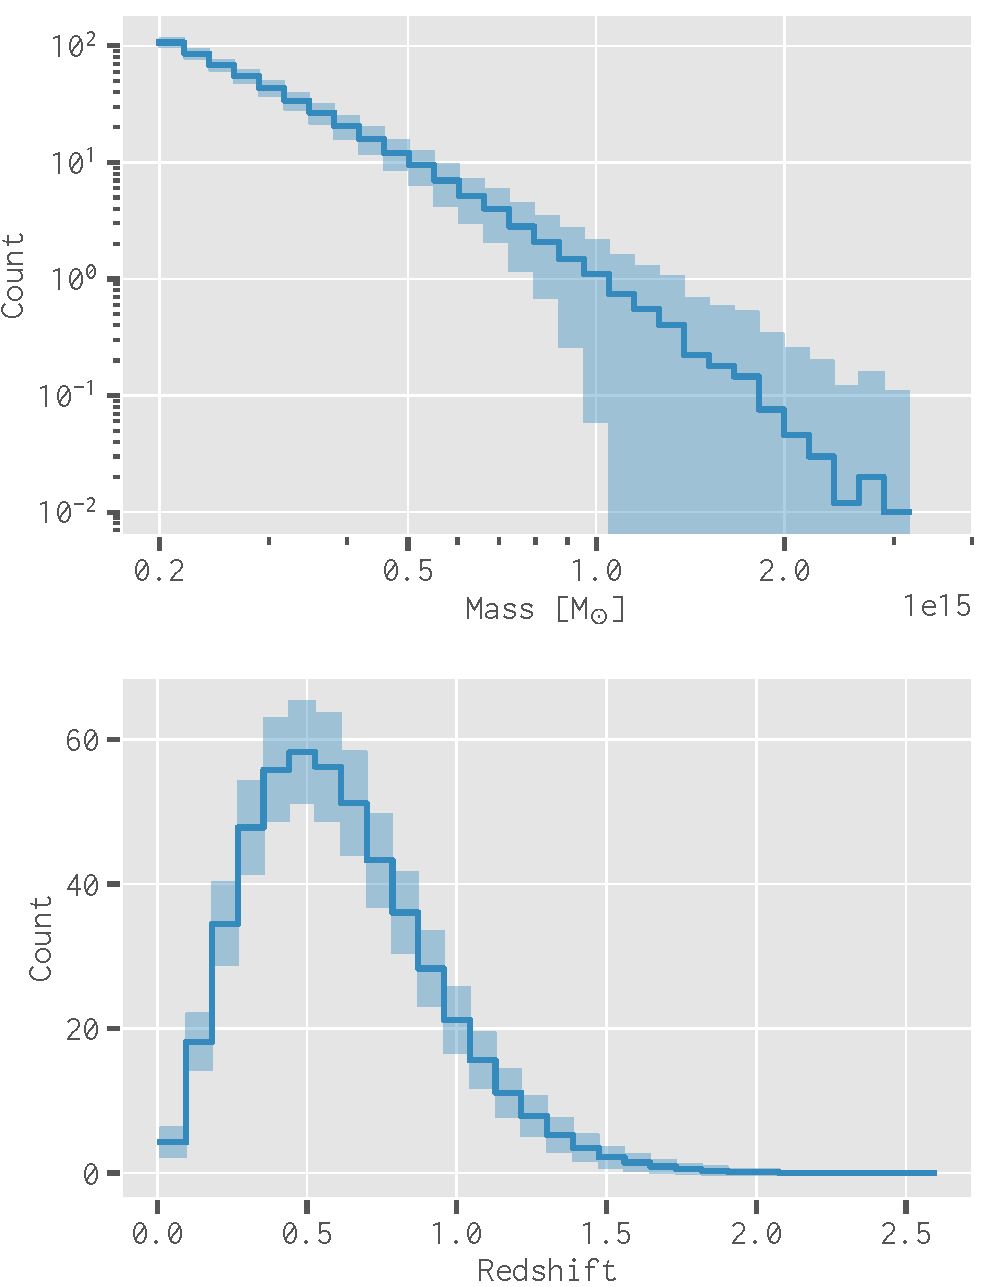
\includegraphics[width=0.8\textwidth]{mass-z-dist}
  \bicaption[星系团的红移和质量分布直方图]{%
    在 \SI{10 x 10}{\degree} 的天区内,星系团的红移(上栏)和质量(下栏)分布直方图.
    其中的实线和阴影区域分别表示 500 次模拟的平均值和 68\% 误差范围.
  }{%
    The mass (upper panel) and redshift (lower panel) histograms of the
    simulated galaxy clusters in a \SI{10 x 10}{\degree} sky patch.
    The solid lines and shaded regions represent the means and
    68\% uncertainties derived from 500 simulation runs,
    respectively.
  }
  \label{fig:m-z-dist}
\end{figure}

%---------------------------------------------------------------------
\subsection{并合历史}
\label{sec:merging-history}

上述 Press--Schechter 质量函数只给出了在不同红移处宇宙中的\ac{gc}的质量分布,
没有提供单个星系团的形成历史.
这个问题由 \citeay{lacey1993} 通过对 Press--Schechter
理论进行了扩展而给出了解决方案.
给定一个星系团,\uline{扩展 Press--Schechter 理论}描述了其\ac{progenitor}的质量分布,
然后利用 Monte Carlo 模拟便可构建出该星系团的成长历史,即\emph{\acf{m-tree}}
\cite{lacey1993,randall2002}.

设一个星系团在 $t_1$ 时刻的质量为 $M_1$,经过一次成长步骤(并合或\ac{accretion})后,
其质量在 $t_2$ ($> t_1$) 时刻增长为 $M_2$.
给定 $M_2$ 和 $t_2$,扩展 Press--Schechter 理论给出了该星系团在一个较早时刻 $t_1$
具有一个质量范围为 $[M_1,\, M_1+\D{M_1}]$ 的\ac{progenitor}的\ac{pr-cond}为
\cite{lacey1993,randall2002}:
\begin{equation}
  \label{eq:eps-condprob}
  \R{Pr}(M_1, t_1 \,|\, M_2, t_2) \,\D{M_1} =
    \frac{1}{\sqrt{2\Cpi}} \frac{M_2}{M_1}
    \frac{\delta_{c1} - \delta_{c2}}{(\sigma_1^2 - \sigma_2^2)^{3/2}}
    \left| \diff{\sigma_1^2}{M_1} \right|
    \exp \!\left[ -\frac{(\delta_{c1} - \delta_{c2})^2}
      {2(\sigma_1^2 - \sigma_2^2)} \right] \,\D{M_1} ,
\end{equation}
其中
$\delta_{ci} \equiv \delta_c(t_i)$,$\sigma_i \equiv \sigma(M_i)$,
同时下标 $i = 1, 2$ 分别表示这些参数在时刻 $t_1$ 和 $t_2$ 的值.
进一步定义 $\psi \equiv \sigma^2(M)$ 和 $\omega \equiv \delta_c(t)$,
上式可简化为:
\begin{equation}
  \label{eq:eps-condprob2}
  \R{Pr}(\Delta\psi, \Delta\omega) \,\D{\Delta\psi} =
    \frac{1}{\sqrt{2\Cpi}} \frac{\Delta\omega}{(\Delta\psi)^{3/2}}
    \exp \!\left[ -\frac{(\Delta\omega)^2}{2 \Delta\psi} \right]
    \,\D{\Delta\psi} ,
\end{equation}
其中
$\Delta\psi = \sigma_1^2 - \sigma_2^2$,
$\Delta\omega = \delta_{c1} - \delta_{c2}$.
注意 $\psi$ 随 $M$ 的增大而单调递减,$\omega$ 亦随 $t$ 的增大而单调递减.

对于样本 (\autoref{sec:mass-function}) 中的每一个星系团,为了模拟其\ac{m-tree},
我们从\enquote{当前的}质量 $M_{\R{sim}}$ 和红移 $z_{\R{sim}}$ 出发,
运用 Monte Carlo 方法逐步追溯其成长历史,时间步长为 $\Delta\omega$.
为了能够分辨质量变化为 $\Delta M_c$ ($\ll M_2$) 的并合,
时间步长 $\Delta\omega$ 应满足 \cite{lacey1993}:
\begin{equation}
  \Delta\omega \lesssim (\Delta\omega)_{\R{max}} =
    \left[ \psi \left| \diff{\ln \sigma^2}{\ln M_2} \right|
      \left( \frac{\Delta M_c}{M_2} \right) \right]^{1/2} .
\end{equation}
本工作采用了自适应的时间步长 \cite{randall2002}:
$\Delta\omega = (\Delta\omega)_{\R{max}} \big/ 2$.

在追溯的每一步,当确定时间步长 $\Delta\omega$ 后,
则并入星系团的质量(由 $\Delta\psi$ 描述)的\ac{cdf}为:
\begin{align}
  F_{\Delta\psi}(<\!\Delta\psi, \Delta\omega)
    & = \int_0^{\Delta\psi} \R{Pr}(\Delta\psi', \Delta\omega)
      \,\D{\Delta\psi'} \\
    & = 1 - \erf \left( \frac{\Delta\omega}{\sqrt{2\Delta\psi}} \right) ,
  \label{eq:cdf-submass}
\end{align}
其中 $\erf(\cdot)$ 为\ac{errfunc}:
\begin{equation}
  \erf(x) = \frac{2}{\sqrt{\pi}} \int_0^x \Ce^{-t^2} \,\D{t} .
\end{equation}
对\autoref{eq:cdf-submass} 随机采样得到一个 $\Delta\psi$,
于是,星系团 $M_2$ 的一个\ac{progenitor}的质量 $M_1$
由 $\psi_1 = \psi_2 + \Delta\psi$ 确定 [参见\autoref{eq:sigma-mass}],
同时另一个\ac{progenitor}的质量为 $\Delta M = M_2 - M_1$.

设 $M_m \equiv \max(M_1, \Delta M)$ 和 $M_s \equiv \min(M_1, \Delta M)$
分别为并合的主星系团(简称\emph{主团})和子星系团(简称\emph{子团}),
如果 $M_s > \Delta M_c$,则认为发生了一次并合事件,否则认为是\ac{accretion}过程
\cite{randall2002}.
目前普遍认为可观测到的\ac{rh}与最近(在观测者的参考系)发生的\ac{m-major}相关联,
而且\ac{rh}的典型寿命较短,比如在 \SI{1.4}{\GHz} 的寿命
$\tau_{\R{halo}} \lesssim \SI{1}{\Gyr}$ \cite{brunetti2009,cassano2016}.
因此,本文采用 $\Delta M_c = \SI{e13}{\solarmass}$ \cite{cassano2005},
并且只针对主团从\enquote{当前}时刻 $t_{\R{sim}}$ (对应于 $z_{\R{sim}}$)
追溯 $t_{\R{back}} = \SI{3}{\Gyr}$.
于是,获得每个星系团的并合历史
$\left\{\left( M_m^{(i)}, M_s^{(i)}, t_{\R{merger}}^{(i)} \right)\right\}$
用于开展后续射电晕的模拟.

星系团的并合历史(即\ac{m-tree})是随机模拟的.
以一个质量为 \SI{e15}{\solarmass} 的星系团为例,重复模拟其\ac{m-tree} 30 次,
可得到 30 颗不同的\ac{m-tree},如\autoref{fig:merging-history} 上栏所示.
同时,该图下栏显示了从 \autoref{sec:mass-function} 样本中随机挑选的 30 个星系团
的\ac{m-tree},其中每个星系团只随机生成了一颗\ac{m-tree}.

\begin{figure}[htp]
  \centering
  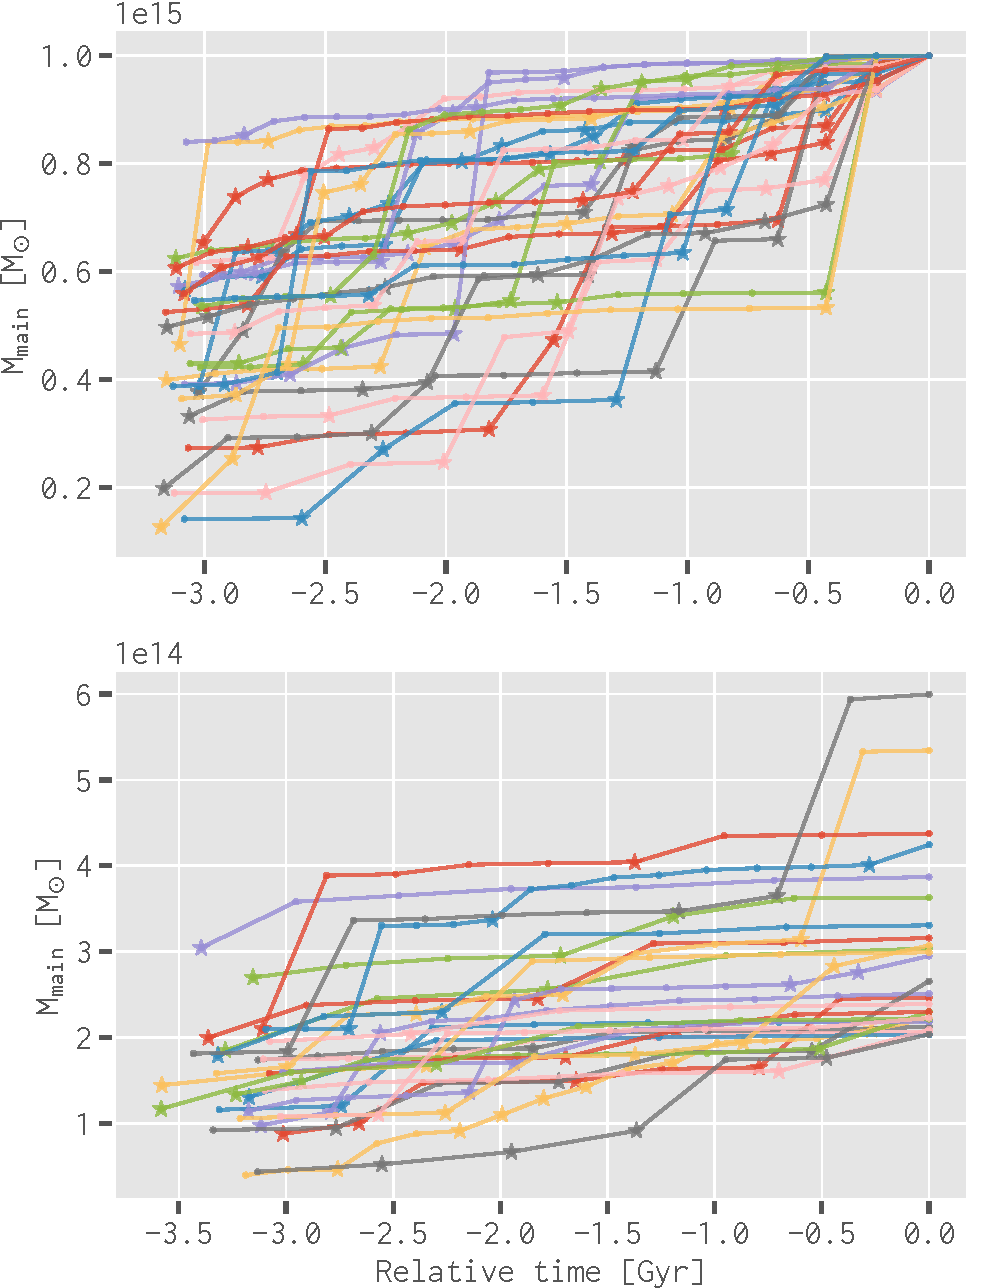
\includegraphics[width=0.8\textwidth]{merging-history}
  \bicaption[星系团并合树的模拟结果示例]{%
    \uline{(上栏)}
    对同一个质量为 \SI{e15}{\solarmass} 的星系团,重复模拟其\acs*{m-tree} 30 次
    所得到的 30 颗不同的\acs*{m-tree}.
    \uline{(下栏)}
    从 \autoref{sec:mass-function} 样本中随机挑选 30 个星系团,
    对每个星系团随机模拟一颗\acs*{m-tree}.
    星号和细点分别表示并合和\acs*{accretion}事件.
  }{%
    \textbf{(Upper)} Merger trees for one galaxy cluster of mass
    \SI{e15}{\solarmass} obtained by repeating the random build process
    for 30 times.
    \textbf{(Lower)} Example merger trees for 30 galaxy clusters randomly
    drawn from the sample constructed in \autoref{sec:mass-function}.
    Asterisks mark merger events and dots represent accretion events.
  }
  \label{fig:merging-history}
\end{figure}

%---------------------------------------------------------------------
\subsection{演化模型}
\label{sec:halo-evo}

根据\ac{turbreacc-model},星系团 \ac{icm} 里充满一群非热的\ac{e-primary},
这些电子可在多种过程中产生并被注入到 \ac{icm} 中,比如 \ac{agn} 活动、恒星形成,
详见 \citeay{blasi2007} 和 \citeay{brunetti2014} 综述文.
当星系团经历\ac{m-major}时,整个 \ac{icm} 中都将产生剧烈的\ac{turbulence},
就地加速\ac{e-primary}至极高的能量 ($\ac{g} > \num{e3}$),
从而形成弥散的\ac{rh}.
在另一方面,多种机制会使这些高能电子损失能量 \cite{sarazin1999},其中包括:
产生\ac{rad-syn}、与 \ac{cmb} 光子发生逆 Compton 散射、
与 \ac{icm} 中的离子发生 Coulomb 碰撞.

对于一群能量分布各向同性的电子,在上述加速和能量损失的共同作用,
其能谱 \ac{n-e} 随时间的演化由以下 Fokker--Planck 方程描述
\cite{eilek1991,schlickeiser2002}:
\begin{equation}
  \label{eq:fokkerplanck}
  \pdiff{\ac{n-e}}{t} =
    \pdiff{}{\ac{g}} \left[ \ac{n-e} \left(
      \left| \diff{\ac{g}}{t} \right| -
      \frac{2}{\ac{g}} \ac{coef-diffusion}(\ac{g}, t) \right) \right]
    + \pdiff{}{\ac{g}} \left[
      \ac{coef-diffusion} \pdiff{\ac{n-e}}{\ac{g}} \right]
    + \ac{e-inj}(\ac{g}, t) ,
\end{equation}
其中
\ac{g} 是电子的 \acl{g},
\ac{coef-diffusion} 是描述\ac{turbulence}和电子相对作用的\acl{coef-diffusion},
$|\R{d}\gamma / \R{d}t|$ 是电子的能量损失速率,
还有 \ac{e-inj} 描述了电子的注入过程.

%.....................................................................
\subsubsection{热成分的性质}

对于星系团 \ac{icm} 的热成分,其中的热电子的数密度 (number density) \ac{n-th} 为:
\begin{equation}
  \label{eq:n-th}
  \ac{n-th} \simeq
    \frac{3 \ac{f-gas} \ac{M-vir}}{
      4\Cpi \ac{mol-weight-m} \ac{mass-u} \,r^3_{\R{vir}}} ,
\end{equation}
其中
$\ac{mol-weight-m} \simeq 0.6$ 是 \ac{icm} 的\acl{mol-weight-m}
(mean molecular weight) \cite{ettori2013},
\ac{mass-u} 是\acl{mass-u} (atomic mass unit),
\ac{M-vir} 是星系团的\acl{M-vir} (virial mass),
\ac{r-vir} 是其\acl{r-vir} (virial radius)
[参见\autoref{eq:radius-virial}],
以及 $\ac{f-gas} \simeq \ac{Ob0}/\ac{Om0}$
是星系团中的气体占总质量 (\ac{M-vir}) 的比例.

相应地,\ac{icm} 的热能密度 (thermal energy density) \ac{e-th} 由下式给出:
\begin{equation}
  \label{eq:e-th}
  \ac{e-th} = \frac{3}{2} \,\ac{n-th} \ac{kb} \ac{T-cl} ,
\end{equation}
其中 \ac{icm} 的平均温度 \ac{T-cl} 可近似为 \cite{cavaliere1998}:
\begin{equation}
  \label{eq:t-icm}
  \ac{T-cl} \simeq \ac{T-vir} + \frac{3}{2} \,T_{\R{out}} ,
\end{equation}
其中 \ac{T-vir} 为星系团的\acl{T-vir} (virial temperature):
\begin{equation}
  \ac{T-vir} =
    \frac{\ac{mol-weight-m} \ac{mass-u} \ac{G} \ac{M-vir}}{2\,\ac{r-vir}} ,
\end{equation}
以及 $T_{\R{out}} \simeq \SI{0.5}{\keV}$
是从星系团外围区域 ($\gtrsim \ac{r-vir}$) 流入的气体的温度 \cite{fujita2003}.

%.....................................................................
\subsubsection{电子注入过程}

星系团及其成员星系中持续发生着 \ac{agn} 活动、恒星形成等过程,
不断地将\ac{e-primary}注入到 \ac{icm} 之中.
因此,可以假定\ac{e-primary}的注入速率 \ac{e-inj-rate} 是恒定的
\cite{cassano2005,donnert2014},
同时还可假定注入电子的能谱为幂律形式 \cite{sarazin1999},于是有:
\begin{equation}
  \label{eq:electron-inj}
  \ac{e-inj}(\ac{g}, t)
    \simeq \ac{e-inj}(\ac{g})
    = \ac{e-inj-rate} \,\ac{g}^{-s} ,
\end{equation}
其中 $s$ 为谱指数,在本工作中设为 2.5 \cite{cassano2005}.

进一步假定注入电子的总能量密度与 \ac{icm} 热能密度 \ac{e-th} 之比为
\ac{f-injection} \cite{cassano2005},可得:
\begin{equation}
  \tau_{\R{cl}} \int_{\ac{g}_{\R{min}}}^{\ac{g}_{\R{max}}}
  \ac{e-inj}(\ac{g}') \,\ac{g}'\ac{e-electron} \,\D{\ac{g}'}
    = \ac{f-injection} \,\ac{e-th} ,
\end{equation}
其中
$\tau_{\R{cl}} \simeq t_{\R{sim}}$
是星系团\enquote{当前}(对应于红移 $z_{\R{sim}}$)的年龄,
\ac{e-electron} 是\acl{e-electron} (rest energy).
考虑到 $\ac{g}_{\R{min}} \ll \ac{g}_{\R{\max}}$,
于是可推导出电子的注入速率 \ac{e-inj-rate} 为:
\begin{equation}
  \label{eq:injrate}
  \ac{e-inj-rate} \simeq
    \frac{(s-2)\,\ac{f-injection}\,\ac{e-th}}{
      \ac{e-electron}\,\tau_{\R{cl}}} \ac{g}_{\R{min}}^{s-2} .
\end{equation}

%.....................................................................
\subsubsection{剥离半径}

When a sub-cluster merges into the main cluster, the gas at its outer
regions is stripped due to the ram pressure \cite{gunn1972}.
The stripping radius \ac{r-strip} of the sub-cluster, outside which the
stripping is efficient, can be obtained from the equipartition between
the ram pressure and the hydrostatic pressure \cite{cassano2005}, i.e.,
\begin{equation}
  \label{eq:rs-eqp}
  \bar{\rho}_m v_{\R{imp}}^2
    = \frac{\rho_s(\ac{r-strip})}{\mu m_u} k_B T_{\R{cl,s}},
\end{equation}
where
$\bar{\rho}_m = \mu m_u n_{\R{th,m}}$ is the mean gas density of the main
cluster,
$v_{\R{imp}}$ is the impact velocity of the two merging clusters,
and $\rho_s(r)$ and $T_{\R{cl,s}}$ are the gas density profile and
temperature of the sub-cluster, respectively.

Starting from a sufficiently large distance with zero velocity,
the impact velocity $v_{\R{imp}}$ of two merging clusters with
masses $M_{\R{vir,m}}$ and $M_{\R{vir,s}}$ is given by
\cite{sarazin2002,cassano2005}
\begin{equation}
  \label{eq:v-imp}
  v_{\R{imp}} \simeq \left[
    \frac{2G (M_{\R{vir,m}} + M_{\R{vir,s}})}{r_{\R{vir,m}}}
    \left( 1 - \frac{1}{\eta_v} \right)\right]^{1/2},
\end{equation}
where $\eta_v \simeq 4 \,(1 + M_{\R{vir,s}}/M_{\R{vir,m}})^{1/3}$.

The gas density profile $\rho_s(r)$ can be well approximated with
a standard $\beta$-model \cite{cavaliere1976}:
\begin{equation}
  \label{eq:beta-model}
  \rho_s(r) = \rho_s(0) \left[1 + (r / r_{\R{c,s}})^2 \right]^{-3\beta/2},
\end{equation}
where
$r_{\R{c,s}}$ and $\beta$ are the core radius and slope parameter,
respectively, and we adopt $r_{\R{c,s}} = 0.1 \,r_{\R{vir,s}}$
\cite{sanderson2003} and
$\beta = 2/3$ \cite{jones1984}.
The central gas density $\rho_s(0)$ can then be determined by the total gas
mass ($M_{\R{gas,s}} = f_{\R{gas}} M_{\R{vir,s}}$).

%.....................................................................
\subsubsection{湍流加速}

The details of interactions between the turbulence and both thermal and
relativistic particles are complicated and still poorly understood.
Among several particle acceleration mechanisms that can be potentially
triggered by the turbulence, the most important one is the transit time
damping process, i.e., the turbulence dissipates its energy and
accelerates particles by interacting with the relativistic particles
(e.g., cosmic rays) in the ICM
(参考 \citeay{brunetti2007} 和 \citeay{brunetti2011} 及其所引文献).
The associated diffusion coefficient is derived to be
\cite{miniati2015,pinzke2017}
\begin{equation}
  \label{eq:dpp}
  D_{\gamma\gamma} = 2 \gamma^2 \zeta \,k_L
    \frac{\langle (\delta v_t)^2 \rangle^2}{\chi_{\R{cr}} \, c_s^3},
\end{equation}
where
$\zeta$ is an efficiency factor characterizing the ICM plasma instabilities
(e.g., due to spatial or temporal intermittency),
$\chi_{\R{cr}} = \epsilon_{\R{cr}} / \epsilon_{\R{th}}$ is the relative
energy density of cosmic rays with respect to the thermal ICM,
$k_L \simeq 2\pi / r_{\R{turb}}$ is the turbulence injection scale
with $r_{\R{turb}}$ being the radius of the turbulence region,
$\langle (\delta v_t)^2 \rangle$ is the turbulence velocity dispersion,
and $c_s$ is the sound speed in the ICM
\begin{equation}
  \label{eq:sound-speed}
  c_s = \sqrt{\gamma_{\R{gas}} k_B T_{\R{cl}} / (\mu m_u)}
\end{equation}
with $\gamma_{\R{gas}} = 5/3$ being the adiabatic index
of ideal monatomic gas.

In addition to mergers, mechanisms such as outflows from AGNs and galactic
winds can introduce turbulence in the ICM, which is found to account for
$\lesssim\,$5\% of the thermal energy in the central regions
of relaxed clusters \cite{vazza2011}.
Therefore, the base velocity dispersion $\langle (\delta v_0)^2 \rangle$
of the turbulence in the absence of mergers is
\begin{equation}
  \label{eq:v-turb-base}
  \langle (\delta v_0)^2 \rangle
    = 3 \chi_{\R{turb}} \frac{k_B T_{\R{cl,m}}}{\mu m_u} ,
\end{equation}
where
$\chi_{\R{turb}}$ is the ratio of energy density between the base
turbulence and the thermal ICM.
A merger will contribute a significant part of its energy to the turbulence
and greatly increase the turbulence velocity dispersion
$\langle (\delta v_t)^2 \rangle$, which leads to
\begin{equation}
  \label{eq:energy-turb}
  E_{\R{turb}} =
    \frac{1}{2} M_{\R{turb}} \langle (\delta v_t)^2 \rangle =
    \frac{1}{2} M_{\R{turb}} \langle (\delta v_0)^2 \rangle + \eta_t E_m ,
\end{equation}
where
$E_m$ is the energy injected by the sub-cluster during the merger,
$\eta_t$ is the fraction of injected energy ($E_m$) transferred into
turbulent waves,
and $M_{\R{turb}}$ is the gas mass enclosed in the turbulence region
of radius $r_{\R{turb}}$, i.e.,
\begin{equation}
  \label{eq:mass-turb}
  M_{\R{turb}} = \int_0^{r_{\R{turb}}} \! \rho(r) 4\pi r^2 \,\D{r},
\end{equation}
where $\rho(r)$ is the gas density profile of the merged cluster
characterized by the $\beta$-model [see \autoref{eq:beta-model}].
The injected energy $E_m$ is approximated as the work done by the infalling
sub-cluster, i.e.,
\begin{equation}
  \label{eq:energy-inj}
  E_m \simeq \bar{\rho}_m v_{\R{imp}}^2 V_{\R{turb}},
\end{equation}
with $V_{\R{turb}} \simeq \pi r_s^2 \,r_{\R{vir,m}}$ being the swept volume
\cite{fujita2003,cassano2005}.
Therefore, the turbulence velocity dispersion during a merger is obtained as
\begin{equation}
  \label{eq:v-turb}
  \langle (\delta v_t)^2 \rangle
    = \langle (\delta v_0)^2 \rangle
    + 2 \pi\,\eta_t\, \bar{\rho}_m r_{\R{vir,m}}
      \,\frac{r_s^2 v_{\R{imp}}^2}{M_{\R{turb}}} .
\end{equation}

One remaining parameter is the turbulence region radius $r_{\R{turb}}$,
which is estimated to be
\begin{equation}
  \label{eq:radius-turb}
  r_{\R{turb}} = r_s + r_{\R{c,m}} ,
\end{equation}
where
$r_{\R{c,m}} = 0.1 \,r_{\R{vir,m}}$ is the core radius of the main cluster,
and $r_s$ is the stripping radius of the sub-cluster
[see \autoref{eq:rs-eqp}]
with a value of $\sim \numrange{1}{2} \,r_{\R{c,m}}$
for major mergers ($M_{\R{vir,m}} / M_{\R{vir,s}} \lesssim 3$)
and $< r_{\R{c,m}}$ for minor mergers
($M_{\R{vir,m}} / M_{\R{vir,s}} \sim \numrange{3}{10}$).
This assumption is well consistent with previous simulation studies, which
show that mergers introduce turbulence in regions of radius about
$\numrange{0.1}{0.3} \,r_{\R{vir,m}}$
\cite{vazza2011,vazza2012,miniati2015ss}.
We note that minor mergers can also generate
a relatively large turbulence region of radius about $r_{\R{c,m}}$
due to the core gas sloshing induced by the infalling sub-cluster
\cite{vazza2012}.
However, the generated turbulence by a minor merger is rather weak because
the injected energy $E_m$ is much less than a major one
[see \autoref{eq:energy-inj}].

%.....................................................................
\subsubsection{能量损失过程}

Among the mechanisms through which relativistic electrons
in the ICM can lose energy, we take into account the following three
major mechanisms in this work \cite{sarazin1999}.
The first one is the inverse Compton scattering off the CMB photons,
the energy loss rate of which is
\begin{equation}
  \label{eq:eloss-ic}
  \left( \diff{\gamma}{t} \right)_{\R{IC}} =
    \num{-4.32e-4} \,\gamma^2 (1+z)^4
    \quad [\si{\per\Gyr}].
\end{equation}

Secondly, with the \si{\uG}-level magnetic field permeating the ICM
\cite{govoni2004,ryu2008}, relativistic electrons will
produce synchrotron radiation and lose energy at a rate of
\begin{equation}
  \label{eq:eloss-syn}
  \left( \diff{\gamma}{t} \right)_{\R{syn}} =
    \num{-4.10e-5} \,\gamma^2 \left( \frac{B}{\SI{1}{\uG}} \right)^2
    \quad [\si{\per\Gyr}],
\end{equation}
where $B$ is the magnetic field strength.
We assume that the magnetic field is uniform and its energy density reaches
equipartition with that of cosmic rays, i.e.,
$\epsilon_B = B^2/(8\pi) \simeq \epsilon_{\R{cr}} = \chi_{\R{cr}}\,\epsilon_{\R{th}}$
\cite{beck2005}.

The last mechanism considered is that relativistic electrons interact
with the thermal electrons via Coulomb collisions, the energy loss rate
of which is
\begin{equation}
  \label{eq:eloss-coul}
  \left( \diff{\gamma}{t} \right)_{\R{Coul}} =
    \num{-3.79e4} \left( \frac{n_{\R{th}}}{\SI{1}{\per\cm\cubed}} \right)
    \left[ 1 + \frac{1}{75} \ln \left(
        \gamma \,\frac{\SI{1}{\per\cm\cubed}}{n_{\R{th}}} \right) \right]
    \quad [\si{\per\Gyr}].
\end{equation}

The inverse Compton scattering and synchrotron radiation dominate
the energy losses at the high-energy regime ($\gamma \gtrsim 1000$),
while Coulomb collisions are the main energy-loss mechanism for electrons
with lower energies ($\gamma \lesssim 100$).
Therefore, electrons with intermediate energies (e.g., $\gamma \sim 300$)
have a long lifetime (\SI{\sim 3}{\Gyr}) and can accumulate in the ICM
as the cluster grows \cite{sarazin1999}.

%---------------------------------------------------------------------
\subsection{数值实现}
\label{sec:numerical}

In order to solve the Fokker--Planck equation [\autoref{eq:fokkerplanck}],
we apply an efficient numerical method proposed by \citeay{chang1970}
and adopt the no-flux boundary condition \cite{park1996}.
To avoid the unphysical pile-up of electrons around the lower boundary
caused by the boundary condition,
we define a buffer region below $\gamma_{\R{buf}}$, within which
the spectral data are replaced by extrapolating the data above
$\gamma_{\R{buf}}$ as a power-law spectrum \cite{donnert2014}.
We adopt a logarithmic grid with 256 cells for $\gamma \in [1, 10^6]$,
and let the buffer region span 10 cells.

By making use of the same Fokker--Planck equation but with the
merger-induced turbulent acceleration turned off [i.e., $E_m \equiv 0$ and
$\langle (\delta v_t)^2 \rangle \equiv \langle (\delta v_0)^2 \rangle$
in \autoref{eq:energy-turb}],
the initial electron spectrum $n_e(\gamma, t_0)$ is derived by evolving the
accumulated electron spectrum $\tilde{n}_e(\gamma) = Q_e(\gamma) \,\tau_0$
for \SI{1}{\Gyr} \cite{brunetti2007}, where $\tau_0$ is the
cluster's age at the beginning of the earliest merger.

Although the whole process of a single merger can last for about
\SIrange{2}{3}{\Gyr} \cite{tormen2004,cassano2016}, the period
during which the turbulence is intense enough to effectively accelerate
electrons is relatively short.
An appropriate estimation of the turbulent acceleration period is
$\tau_{\R{turb}} \simeq 2 \,r_{\R{turb}} / v_{\R{imp}}$ \cite{miniati2015}.

A galaxy cluster may experience multiple mergers in the past
$t_{\R{back}} = \SI{3}{\Gyr}$.
For each merger event
$\left( M^{(i)}_{\R{vir,m}}, M^{(i)}_{\R{vir,s}}, t^{(i)}_{\R{begin}} \right)$,
where $t^{(i)}_{\R{begin}}$ denotes the beginning time of this merger,
it can induce effective turbulent acceleration (i.e., being active) during
the period $\left[ t^{(i)}_{\R{begin}}, t^{(i)}_{\R{end}} \right]$ with
$t^{(i)}_{\R{end}} = t^{(i)}_{\R{begin}}+\tau^{(i)}_{\R{turb}}$ being the
time when this merger becomes inactive.
At other times (i.e., no active merger), only the base turbulence
contributes to the acceleration of electrons, which, however,
is insufficient to balance the energy loss due to synchrotron radiation
and inverse Compton scattering.

Along the history of a galaxy cluster that has multiple mergers, the
turbulence region has a different radius during different mergers.
To take this variation into account, we identify the radius of the largest
turbulence region ($R_{\R{turb}}$) and properly diffuse the electron
spectrum to the sphere of radius $R_{\R{turb}}$ for mergers with a smaller
turbulence region.
Specifically, for a merger that is active during 
$\left[ t^{(i)}_{\R{begin}}, t^{(i)}_{\R{end}} \right]$ and has a
turbulence region of radius $r^{(i)}_{\R{turb}}$, the accelerated part of
the electron spectrum during this merger [i.e., the difference between
spectra at $t^{(i)}_{\R{end}}$ and at $t^{(i)}_{\R{begin}}$] is re-scaled
by a volume ratio given by
\begin{equation}
  \label{eq:ratio-v}
  R_{\R{vol}} = \left[ r^{(i)}_{\R{turb}} \,\Big/ R_{\R{turb}} \right]^3 .
\end{equation}

Once the desired electron spectrum $n_e(\gamma, t)$ is obtained, the
synchrotron emissivity at a frequency $\nu$ is given by \cite{rybicki1979}
\begin{equation}
  \label{sec:jnu-sync}
  % unit: [erg/s/Hz/cm^3]
  J(\nu) = \frac{\sqrt{3} \, e^3 B}{m_e c^2}
    \!\int_{\gamma_{\R{min}}}^{\gamma_{\R{max}}} \!\!\!\int_0^{\pi/2}\!
    n_e(\gamma, t) F(\nu/\nu_c) \sin^2 \!\theta \,\D{\theta} \,\D{\gamma},
\end{equation}
where
$c$ is the speed of light,
$e$ is the elementary charge,
$\theta$ is the pitch angle of electrons with respect to the magnetic
field, $\nu_c = (3/2) \,\gamma^2 \nu_L \sin\theta$ is the electron's
critical frequency with $\nu_L = e B / (2\pi m_e c)$ being the Larmor
frequency, and $F(\cdot)$ is the synchrotron kernel:
\begin{equation}
  \label{eq:sync-kernel}
  F(x) = x \int_x^{\infty} K_{5/3}(y) \,\D{y} ,
\end{equation}
where $K_{5/3}(\cdot)$ is the modified Bessel function of 5/3 order.

\begin{figure}[htp]
  \centering
  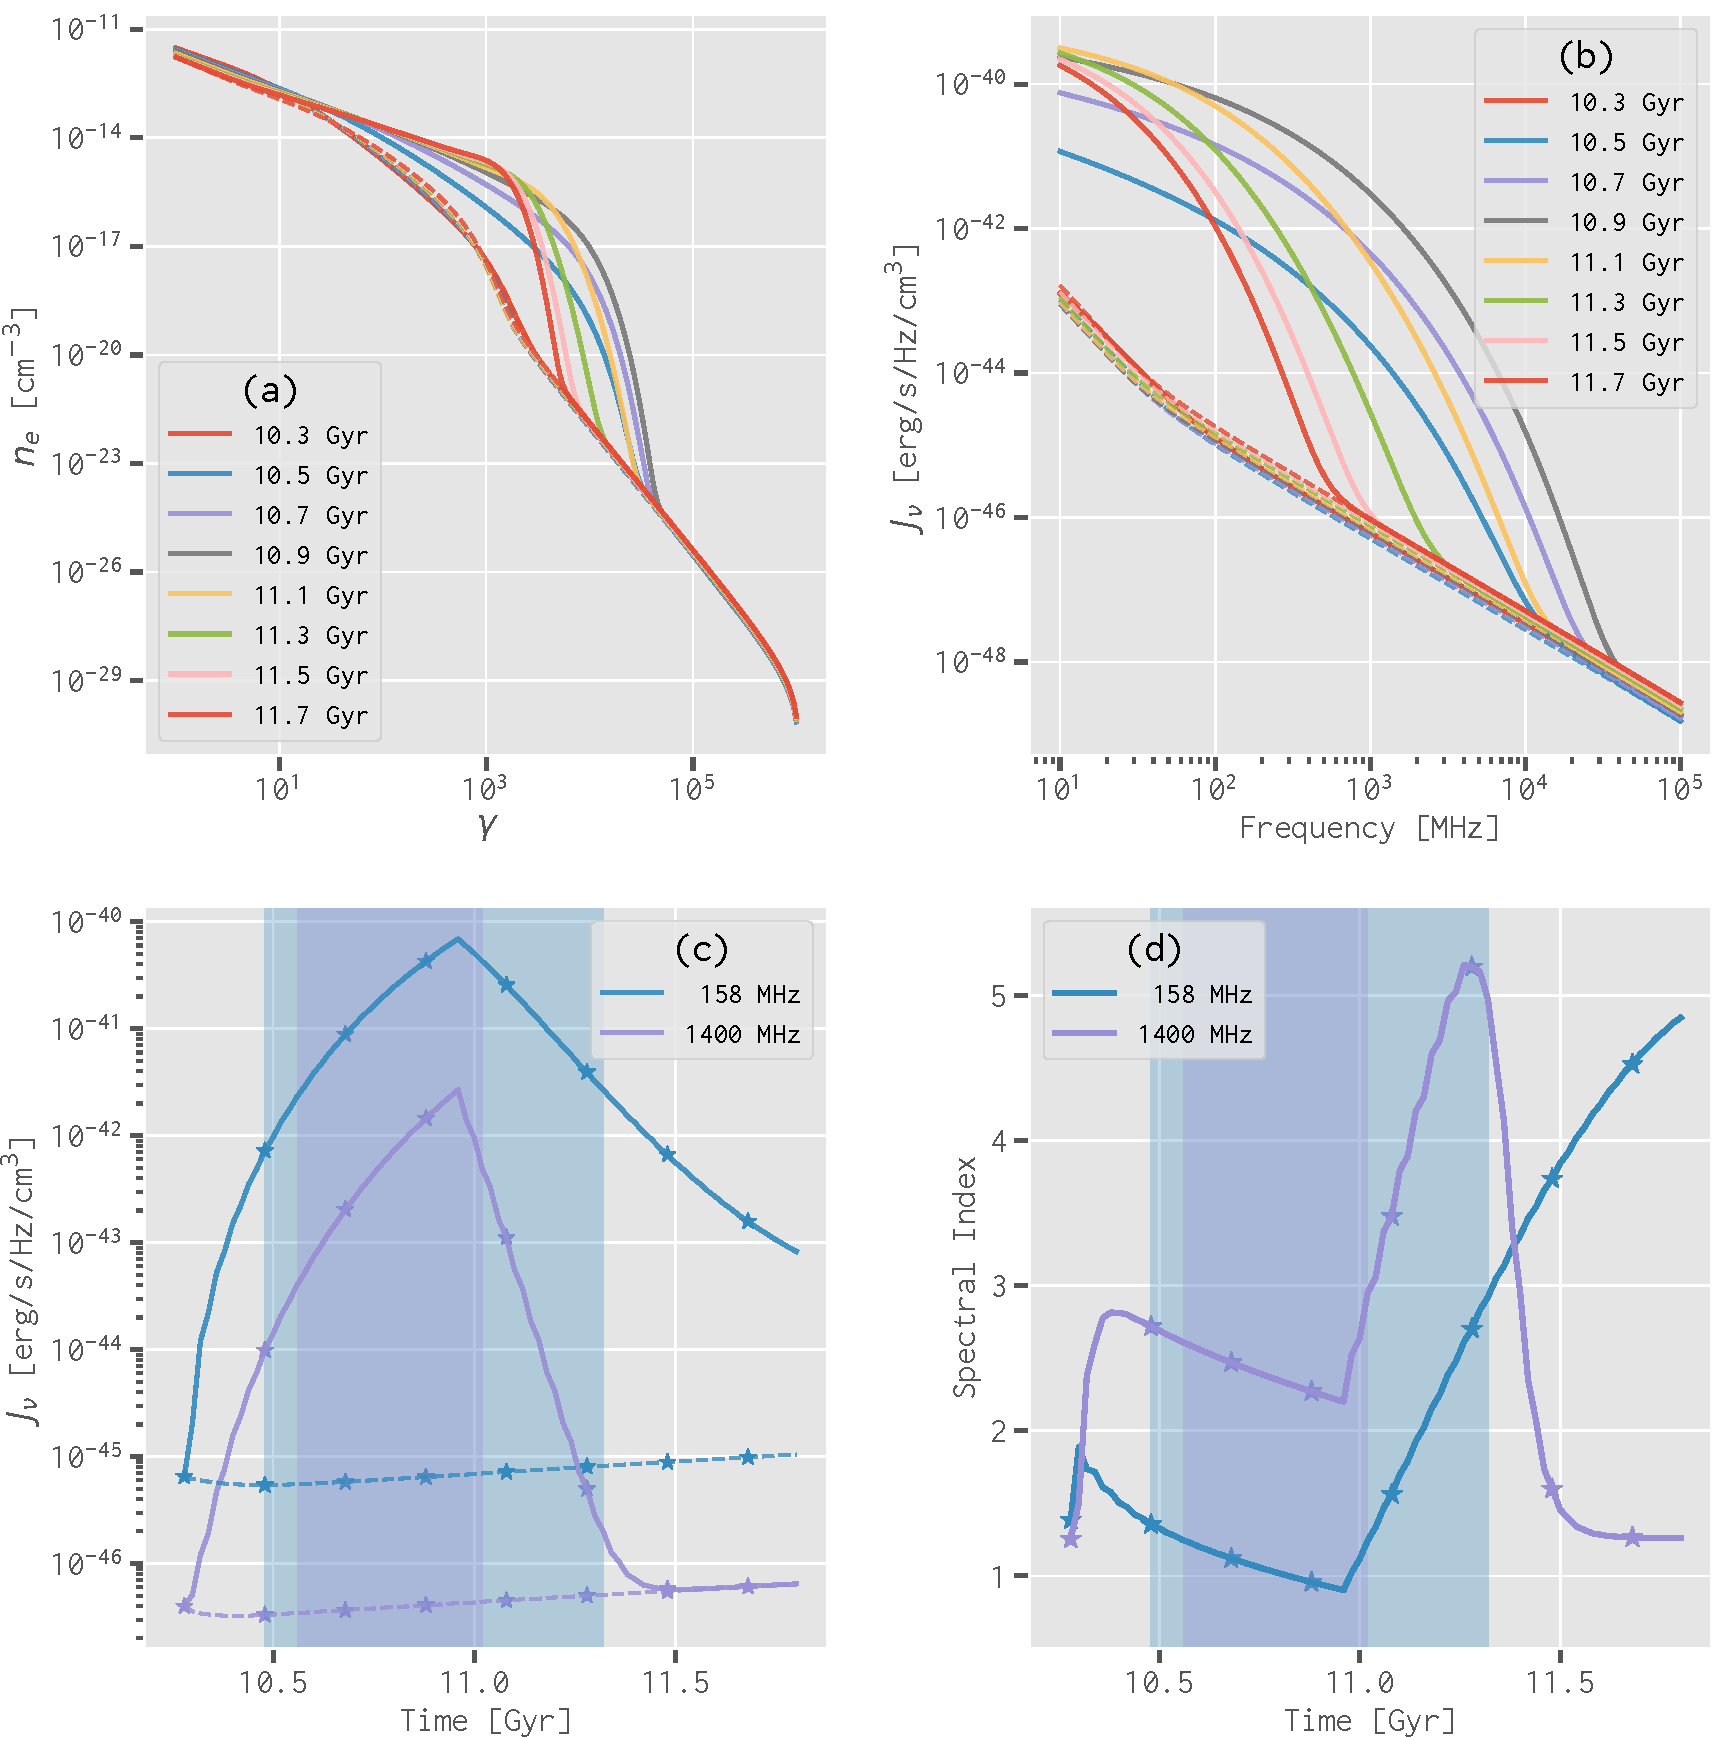
\includegraphics[width=\textwidth]{spec-evo-example}
  \bicaption[电子能谱和同步辐射频谱随时间的演化示例]{%
    TODO...
  }{%
    The temporal evolution of the electron and synchrotron
    emission spectra for an example cluster with one major merger,
    which begins at redshift $z = 0.3$ (i.e., $t \simeq \SI{10.3}{\Gyr}$)
    and is tracked until $z = 0.15$ (i.e., $t \simeq \SI{11.8}{\Gyr}$).
    \textbf{(a)} The relativistic electron spectra (solid lines) and the
    corresponding reference electron spectra (dashed lines; see
    \autoref{sec:halo-size}).
    \textbf{(b)} The synchrotron emission spectra (solid lines) and the
    corresponding reference synchrotron spectra (dashed lines).
    \textbf{(c)} The variation of \SI{158}{\MHz} (solid blue line) and
    \SI{1400}{\MHz} (solid purple line) synchrotron emissivity as well as
    the corresponding reference emissivity (dashed lines) with time.
    \textbf{(d)} The temporal variation of spectral indices at
    \SI{158}{\MHz} (blue line) and \SI{1400}{\MHz} (purple line).
    Shaded regions show the periods during which the radio halo exists
    (see \autoref{sec:halo-size}).
    Asterisks mark the time points corresponding to the spectra presented
    in panels (a) and (b).
  }
  \label{fig:spec-evo}
\end{figure}

In \autoref{fig:spec-evo}, we present the temporal evolution of the
relativistic electron and synchrotron emission spectra for an example
galaxy cluster with one major merger.
The cluster has a mass of \SI{e15}{\solarmass} and merges with a
sub-cluster of mass \SI{6e14}{\solarmass} at redshift $z = 0.3$
(i.e., $t \simeq \SI{10.3}{\Gyr}$), from when we solve the Fokker--Planck
equation to track the electron and synchrotron emission spectra until
redshift $z = 0.15$ (i.e., $t \simeq \SI{11.8}{\Gyr}$).
As demonstrated in this figure, the merger-induced turbulence is active
for a period of $\tau_{\R{turb}} \simeq \SI{0.67}{\Gyr}$ and efficiently
accelerates electrons to extremely high energies
($\gamma \gtrsim \num{e4}$), which gives rise to the radio halo even at
high frequencies ($> \si{\GHz}$).
However, once the turbulence becomes inactive ($t > \SI{10.9}{\Gyr}$), the
high-energy electrons quickly lose energy and the radio halo fades out
shortly, especially at high frequencies.

%---------------------------------------------------------------------
\subsection{识别和大小}
\label{sec:halo-size}

Radio halos cannot form or will rapidly disappear if there is no active
turbulent acceleration.
In order to determine whether or not there exists a radio halo at frequency
$\nu$, we employ the following two criteria:
(1) the synchrotron emissivity $J(\nu)$ of the final electron spectrum
$n_e(\gamma, t_{\R{sim}})$ is at least \num{1000} times larger than the
emissivity $J'(\nu)$ of the reference electron spectrum
$n'_e(\gamma, t_{\R{sim}})$, which is obtained by solving the identical
Fokker--Planck equation but without merger-induced turbulent acceleration,
similar to the way of deriving the initial electron spectrum
(\autoref{sec:numerical});
(2) the spectral index\footnote{%
  We adopt a power-law spectrum of form $J(\nu) \propto \nu^{-\alpha}$.}
at frequency $\nu$ satisfies $\alpha_{\nu} \le 3$.
For the example as shown in \autoref{fig:spec-evo}(c,d), a radio halo
is identified from about 10.6 to 11.0 \si{\Gyr} at \SI{1.4}{\GHz} and
from about 10.5 to 11.3 \si{\Gyr} at \SI{158}{\MHz}.
The spectral indices at \SI{1.4}{\GHz} and \SI{158}{\MHz} reach about 2.1
and 1.0, respectively.
These results demonstrate that radio halos have longer lifetimes at low
frequencies and thus it is expected to observe more radio halos in
low-frequency radio bands.
We note that the \SI{1.4}{\GHz} spectral index ($\alpha_{1400} \sim 2.1$)
is slightly larger than the general result from observations,
because we calculate the spectral index around a specific frequency while
observed spectral indices are generally obtained from two separated
frequencies (e.g., 0.3 and 1.4 GHz \cite{feretti2012}).

Previous studies \cite{cassano2007,basu2012}
have shown that the radius of radio halos ($r_{\R{halo}}$)
increases non-linearly with the cluster's virial radius ($r_{\R{vir}}$),
which may be caused by the distributions of relativistic electrons and
magnetic fields \cite{dolag2002}.
Therefore, we assume the following scaling relation for $r_{\R{halo}}$:
\begin{equation}
  \label{eq:r-halo}
  r_{\R{halo}} = f_r R_{\R{turb}}
    \left( \frac{r_{\R{vir}}}{r_{\R{vir,*}}} \right)^b ,
\end{equation}
where
$R_{\R{turb}}$ is the radius of the largest turbulence region as also used
in \autoref{eq:ratio-v},
$r_{\R{vir,*}}$ is the virial radius of a reference cluster of mass
\SI{e15}{\solarmass},
and $f_r$ and $b$ are the scaling normalization and slope, respectively.
After comparing with the observed scaling relation of
$r_{\R{halo}} \propto r_{\R{vir}}^{2.63 \pm 0.50}$ \cite{cassano2007},
we obtain $f_r = 0.7$ and $b = 1.8$.

Then, the power of a radio halo at frequency $\nu$ is
\begin{equation}
  \label{eq:halo-power}
  P(\nu) = \frac{4\pi}{3} r_{\R{halo}}^3 J(\nu),
\end{equation}
and the flux density at the same frequency is
\begin{equation}
  \label{eq:halo-flux}
  S(\nu) = \frac{(1+z_{\R{sim}}) P(\nu(1+z_{\R{sim}}))}
    {4\pi D_{\!L}^2(z_{\R{sim}})} ,
\end{equation}
where $D_{\!L}(z_{\R{sim}})$ is the luminosity distance to the halo,
and the factor $(1 + z_{\R{sim}})$ accounts for the $K$ correction
\cite{hogg1999}.

%---------------------------------------------------------------------
\subsection{模型参数和结果}
\label{sec:halo-results}

Our model has the following parameters:
(1) $\eta_e$: ratio of the energy density of injected electrons to the
thermal energy density;
(2) $\eta_t$: fraction of the merger energy transferred into the
turbulence;
(3) $\chi_{\R{cr}}$: relative energy density of cosmic rays to the thermal
component;
(4) $\chi_{\R{turb}}$: relative energy density of the base turbulence;
(5) $\zeta$: efficiency of the ICM plasma instabilities.
Since currently no reasonable constraints on these parameters can be
obtained from either observational or theoretical studies,
it is necessary to tune them to make the model predictions (e.g., the halo
flux function, the scaling relation between the halo power and the hosting
cluster mass) consistent with observations.

We perform two comparisons between our simulations and observations.
The first comparison involves the observed scaling relation between the
radio halo power at \SI{1.4}{\GHz} ($P_{1400}$) and the cluster mass
($M_{\R{vir}}$).
We make use of the observation data presented by \citeay{cassano2013},
who reported a scaling relation of
$P_{1400} \propto M_{500}^{3.70 \pm 0.56}$.
We convert their mass $M_{500}$ to virial mass by assuming an NFW density
profile \cite{navarro1997} and employing the mass--concentration relation
derived by \citeay{duffy2008}.
Secondly,
we compare the \SI{1.4}{\GHz} all-sky integrated flux function between
the simulated radio halos and observations.
To this end, we have collected all currently observed radio halos
(\autoref{tab:halos} in \autoref{app:halos};
71 identified halos and 9 candidates; as of 2018 January).
Considering that current observations are far from complete,
especially at the low-flux end, our strategy is to require that the
flux function of simulated radio halos agrees with the
observed one at the high-flux end.

\begin{figure}[htp]
  \centering
  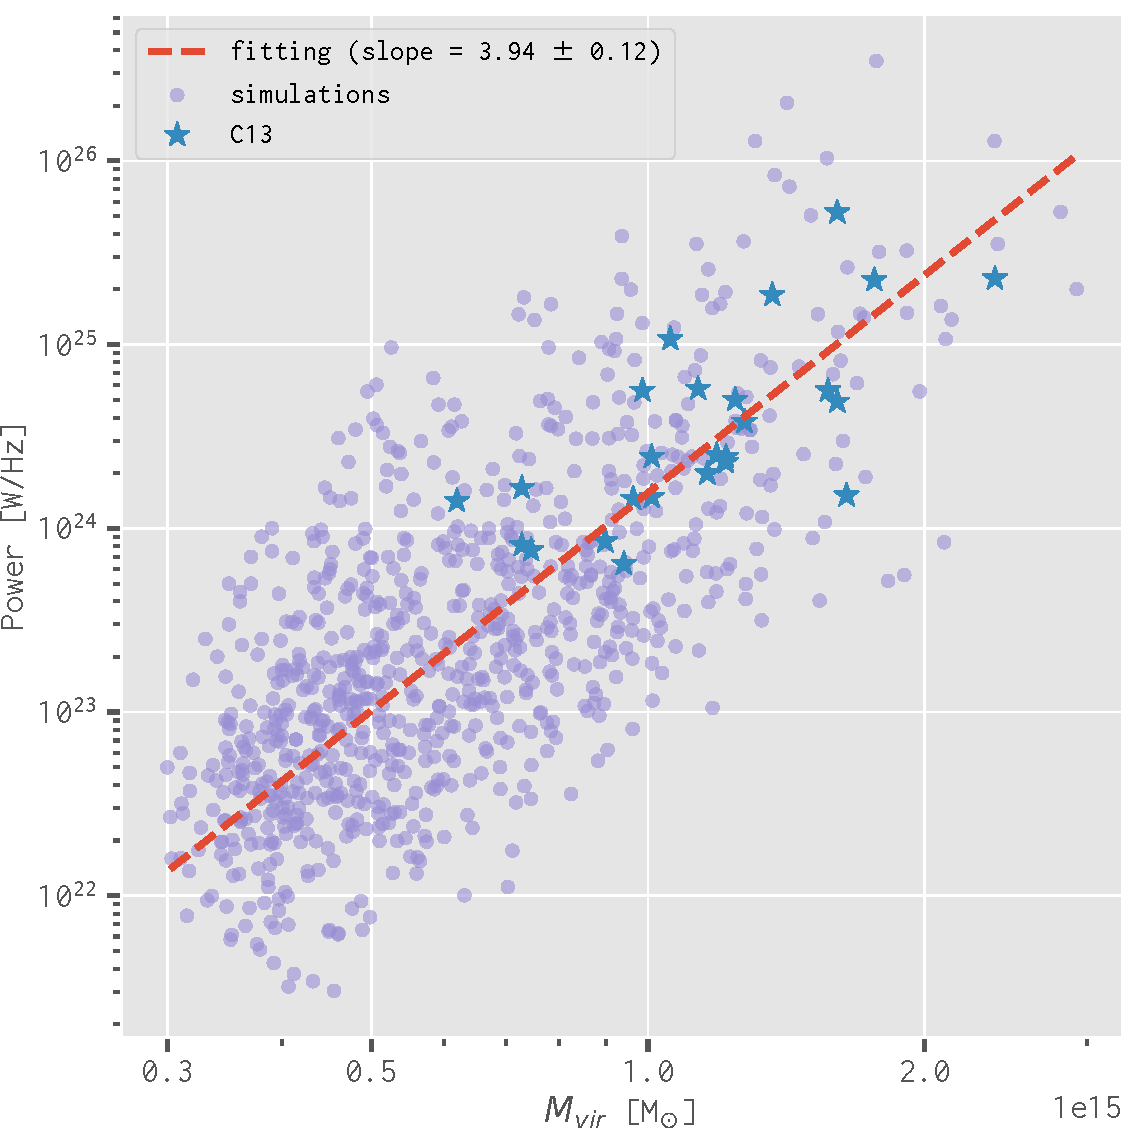
\includegraphics[width=0.8\textwidth]{halo-power-mvir}
  \bicaption[射电晕 \SI{1.4}{\GHz} 功率和宿主星系团质量之间的标度关系]{%
    TODO...
  }{%
    Simulated scaling relation between the radio halo power at
    \SI{1.4}{\GHz} ($P_{1400}$) and the cluster mass ($M_{\R{vir}}$).
    Blue asterisks mark the observation data from \citeay{cassano2013}.
    Purple dots represent the results of 500 simulation runs
    and the dashed red line shows the fitted relation of
    $P_{1400} \propto M_{\R{vir}}^{3.94 \pm 0.12}$.
  }
  \label{fig:halo-power}
\end{figure}

\begin{figure}[htp]
  \centering
  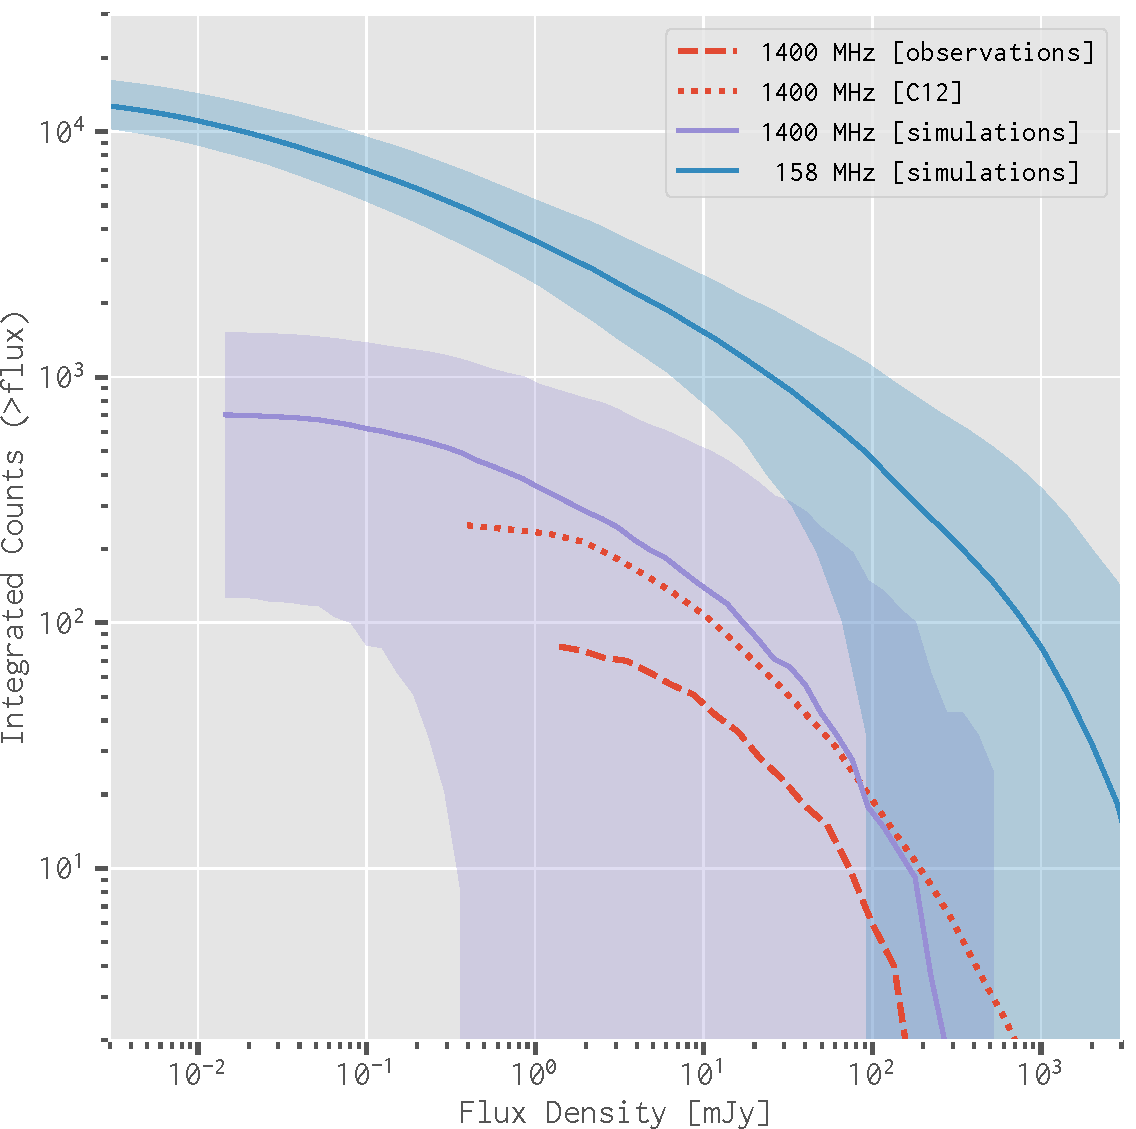
\includegraphics[width=0.8\textwidth]{fluxfunc-simucomp}
  \bicaption[射电晕 \SI{1.4}{\GHz} 流量函数的对比]{%
    TODO...
  }{%
    The \SI{1.4}{\GHz} all-sky integrated flux function comparison
    between the observed (dashed purple line) and simulated
    (solid purple line) radio halos.
    The dotted red line shows the \SI{1.4}{\GHz} flux function
    predicted by \citeay{cassano2012}.
    The solid blue line represents the \SI{158}{\MHz} flux function for
    the simulated halos as a comparison.
    Shaded regions mark the 68\% uncertainties of the
    simulated radio halos estimated from the 500 simulation runs.
  }
  \label{fig:halos-simucomp}
\end{figure}

We have explored various parameter configurations,
and for each configuration we have repeated the simulation for 500 times
in order to take into account the distribution variations of bright
radio halos across the sky.
By comparing the simulation results with the observed
$P_{1400}$--$M_{\R{vir}}$ scaling relation and the \SI{1.4}{\GHz} flux
function, we finally choose a set of model parameters with
$\eta_e = 0.01\%$,
$\eta_t = 15\%$,
$\chi_{\R{cr}} = 1.5\%$,
$\chi_{\R{turb}} = 1.5\%$,
and $\zeta = 0.1$.
As shown in \autoref{fig:halo-power}, the radio halos simulated by our
model with the tuned parameters show a scaling relation of $P_{1400}
\propto M_{\R{vir}}^{3.94 \pm 0.12}$, which is consistent well with that of
\citeay{cassano2013} on both the slope and normalization.
In \autoref{fig:halos-simucomp}, we present the \SI{1.4}{\GHz} flux
functions for the simulated radio halos and observed ones, which agree with
each other at the high-flux end.
The \SI{1.4}{\GHz} flux function given by our tuned model also matches
the prediction of \citeay{cassano2012}.

Furthermore, we display the fraction of clusters with radio halos as a
function of the cluster mass in \autoref{fig:halo-fraction}.
It clearly shows that more massive clusters tend to have higher
probabilities to host radio halos.
Meanwhile, we are expected to observe much more radio halos at low
frequencies (e.g., $\sim \SIrange{100}{200}{\MHz}$), which could be
generated by less intense mergers and have longer lifetimes (see also
\autoref{sec:numerical} and \autoref{fig:spec-evo}).

\begin{figure}[htp]
  \centering
  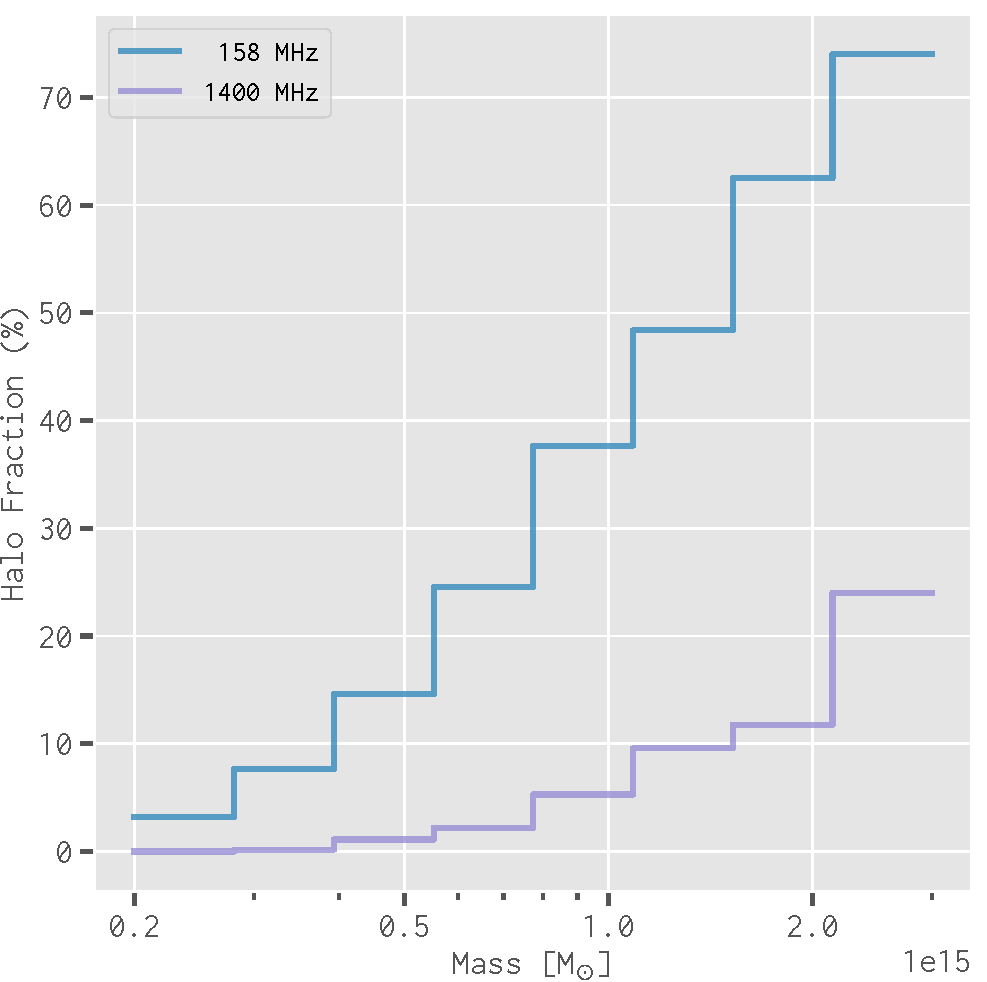
\includegraphics[width=0.8\textwidth]{halo-fraction}
  \bicaption[具有射电晕的星系团比例随星系团质量的变化]{%
    TODO...
  }{%
    The fraction of clusters with radio halos as a function of the cluster
    mass.
    The blue and purple lines represent the fraction of halos identified at
    \SI{158}{\MHz} and \SI{1400}{\MHz}, respectively.
  }
  \label{fig:halo-fraction}
\end{figure}

%---------------------------------------------------------------------
\subsection{图像生成}
\label{sec:halo-maps}

To generate images for the simulated radio halos, we adopt an
exponential profile for the azimuthally averaged brightness distribution
\cite{murgia2009}:
\begin{equation}
  \label{eq:halo-profile}
  I_{\nu}(\theta) = I_{\nu,0} \exp(-3 \,\theta / \theta_{\R{halo}}),
\end{equation}
where $\theta = r / D_{\!A}(z_{\R{sim}})$ is the angular radius from the
halo center with $D_{\!A}(z_{\R{sim}})$ being the angular diameter
distance to the halo,
and $I_{\nu,0} = 9 S(\nu) / (2\pi \theta^2_{\R{halo}})$ is the central
brightness.

In order to characterize the uncertainty of the number density of bright
radio halos across the sky, we repeat the simulation of radio halos
for 100 times.
The medians and the corresponding 68\% uncertainties\footnote{%
  The 68\% uncertainty is derived from the 16$^{\text{th}}$
  and 84$^{\text{th}}$ percentiles because they are more robust than the
  mean and standard deviation for data with large dispersion.}
of the root-mean-square brightness temperature are
$\left(4.21_{-2.60}^{+11.2}\right) \times 10^3$ \si{\mK},
$\left(1.81_{-1.13}^{+5.28}\right) \times 10^3$ \si{\mK}, and
$\left(0.85_{-0.54}^{+2.74}\right) \times 10^3$ \si{\mK}
at \numlist{124; 158; 196} \si{\MHz}, respectively
(\autoref{tab:tb-rms}; see also \autoref{fig:halos-skymap} for an
example map of the simulated radio halos at \SI{158}{\MHz}).

\begin{figure}[htp]
  \centering
  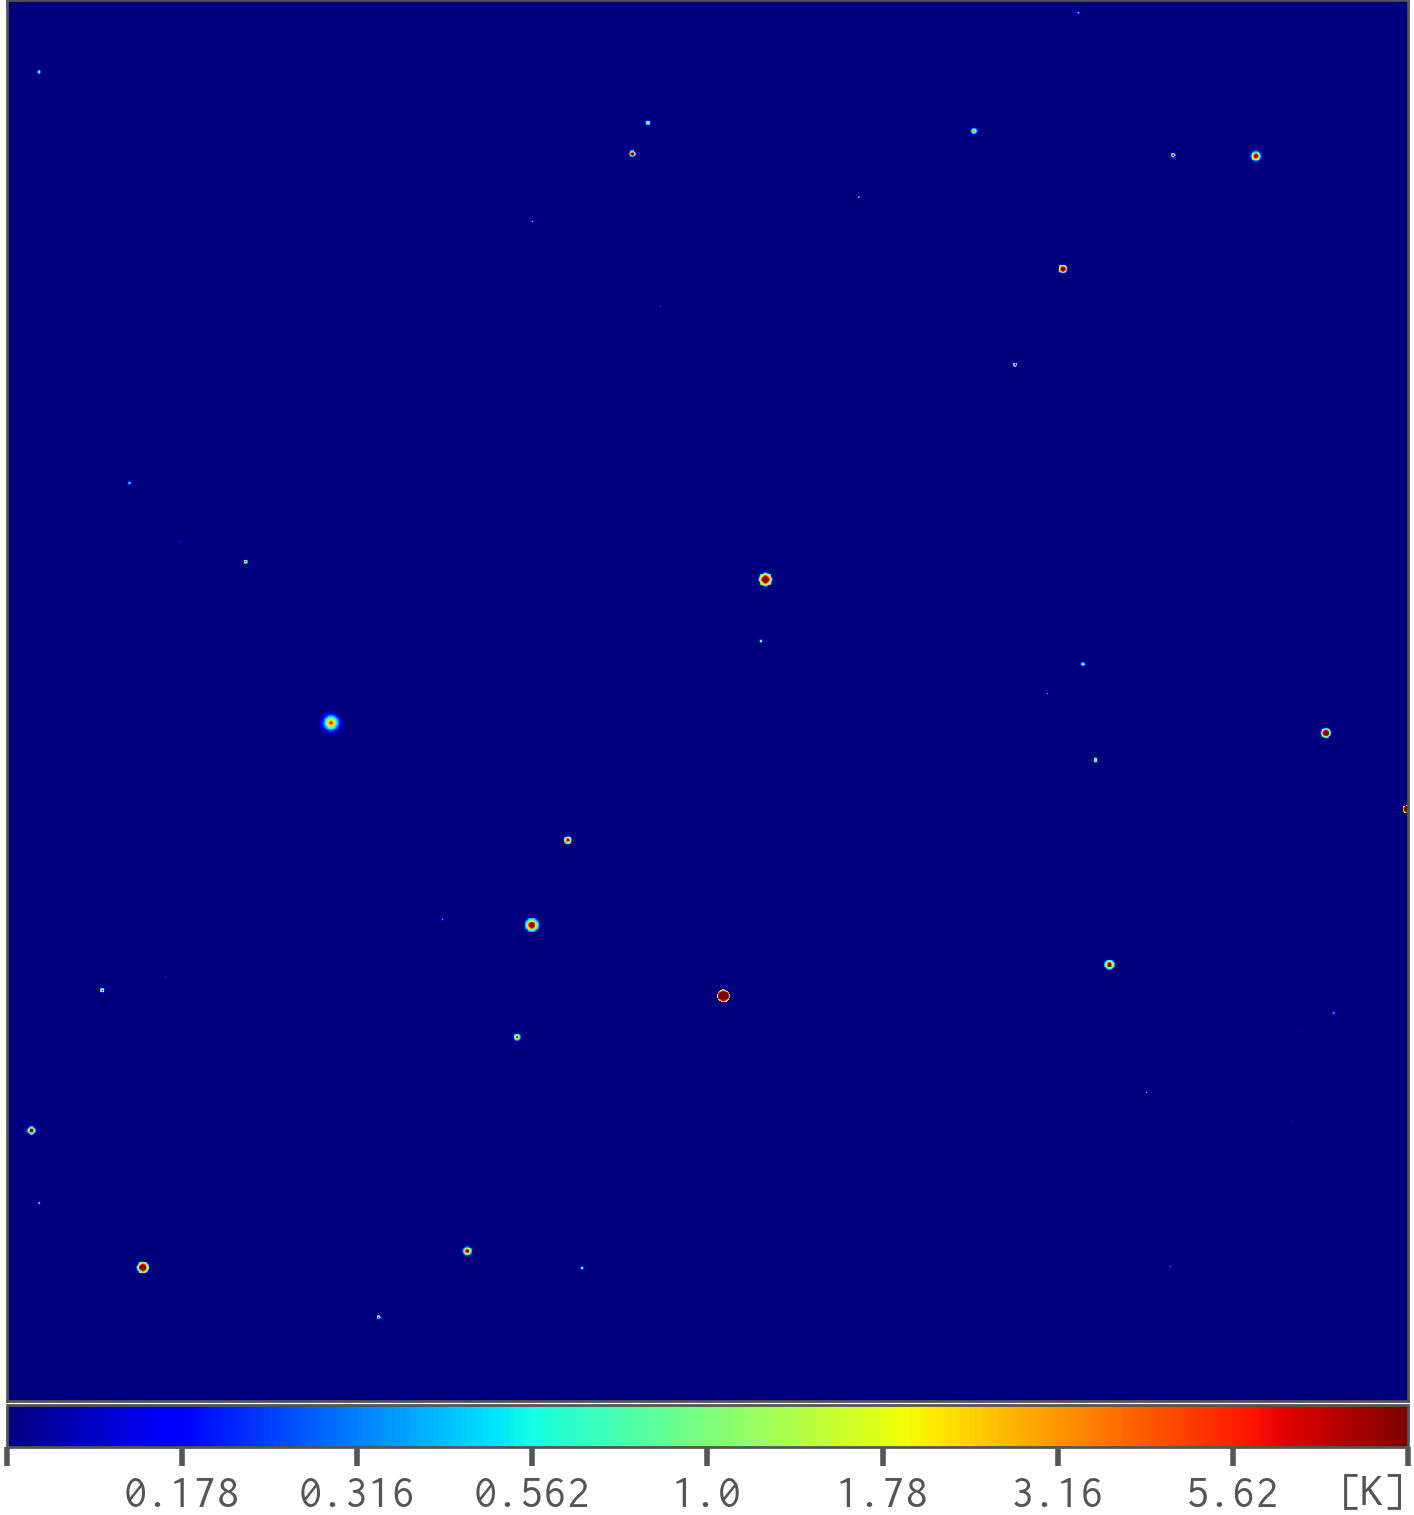
\includegraphics[width=0.8\textwidth]{skymap-halos-f158}
  \bicaption[射电晕在 \SI{158}{\MHz} 的模拟天图示例]{%
    TODO...
  }{%
    An example from the 100 simulation runs showing the simulated
    radio halos at \SI{158}{\MHz}.
    The sky region size is \SI{10 x 10}{\degree},
    and the color bar is in units of \si{\kelvin}.
  }
  \label{fig:halos-skymap}
\end{figure}

\begin{table}[htp]
  \centering
  \bicaption[所有成分的亮温度的\acs*{rms}值]{%
    所有成分的亮温度的\acs*{rms}值(单位: mK)
  }{%
    The Root-Mean-Square Brightness Temperatures of All Components
    (unit: mK)
  }
  \label{tab:tb-rms}

  \begin{tabular}{cccc}
    \toprule
    成分 & \SI{124}{\MHz} & \SI{158}{\MHz} & \SI{196}{\MHz} \\
    \midrule
    射电晕(100 次模拟) &
      $\left(4.21_{-2.60}^{+11.2}\right) \times 10^3$ &
      $\left(1.81_{-1.13}^{+5.28}\right) \times 10^3$ &
      $\left(0.85_{-0.54}^{+2.74}\right) \times 10^3$ \\
    银河系同步辐射 & \num{4.74e5} & \num{2.52e5} & \num{1.43e5} \\
    银河系自由--自由辐射 & \num{330} & \num{200} & \num{130} \\
    河外点源 & \num{29.7e7} & \num{5.90e7} & \num{1.39e7} \\
    EoR 信号 & \num{15.1} & \num{11.3} & \num{3.77} \\
    \bottomrule
  \end{tabular}
\end{table}


%=====================================================================
\section{银河系}

TODO...

%---------------------------------------------------------------------
\subsection{同步辐射}

TODO... simulation details...

The Galactic synchrotron map is simulated by extrapolating the
Haslam \SI{408}{\MHz} all-sky map as the template to lower frequencies
with a power-law spectrum.
We make use of the high-resolution version ($N_{\R{side}} = 2048$,
pixel size \SI{\sim 1.72}{\arcminute}) of the Haslam \SI{408}{\MHz}
map\footnote{The reprocessed Haslam \SI{408}{\MHz} map:
  \url{http://www.jb.man.ac.uk/research/cosmos/haslam_map/}},
which was reprocessed by \citeay{remazeilles2015} using significantly
better instrument calibration and more accurate subtraction of
extragalactic sources.
We also use the all-sky synchrotron spectral index map made by
\citeay{giardino2002} to account for the index variation with sky positions.
\autoref{fig:galactic-skymaps} 左栏显示了银河系\ac{rad-syn}在 \SI{158}{\MHz} 的天图.

\begin{figure}[htp]
  \centering
  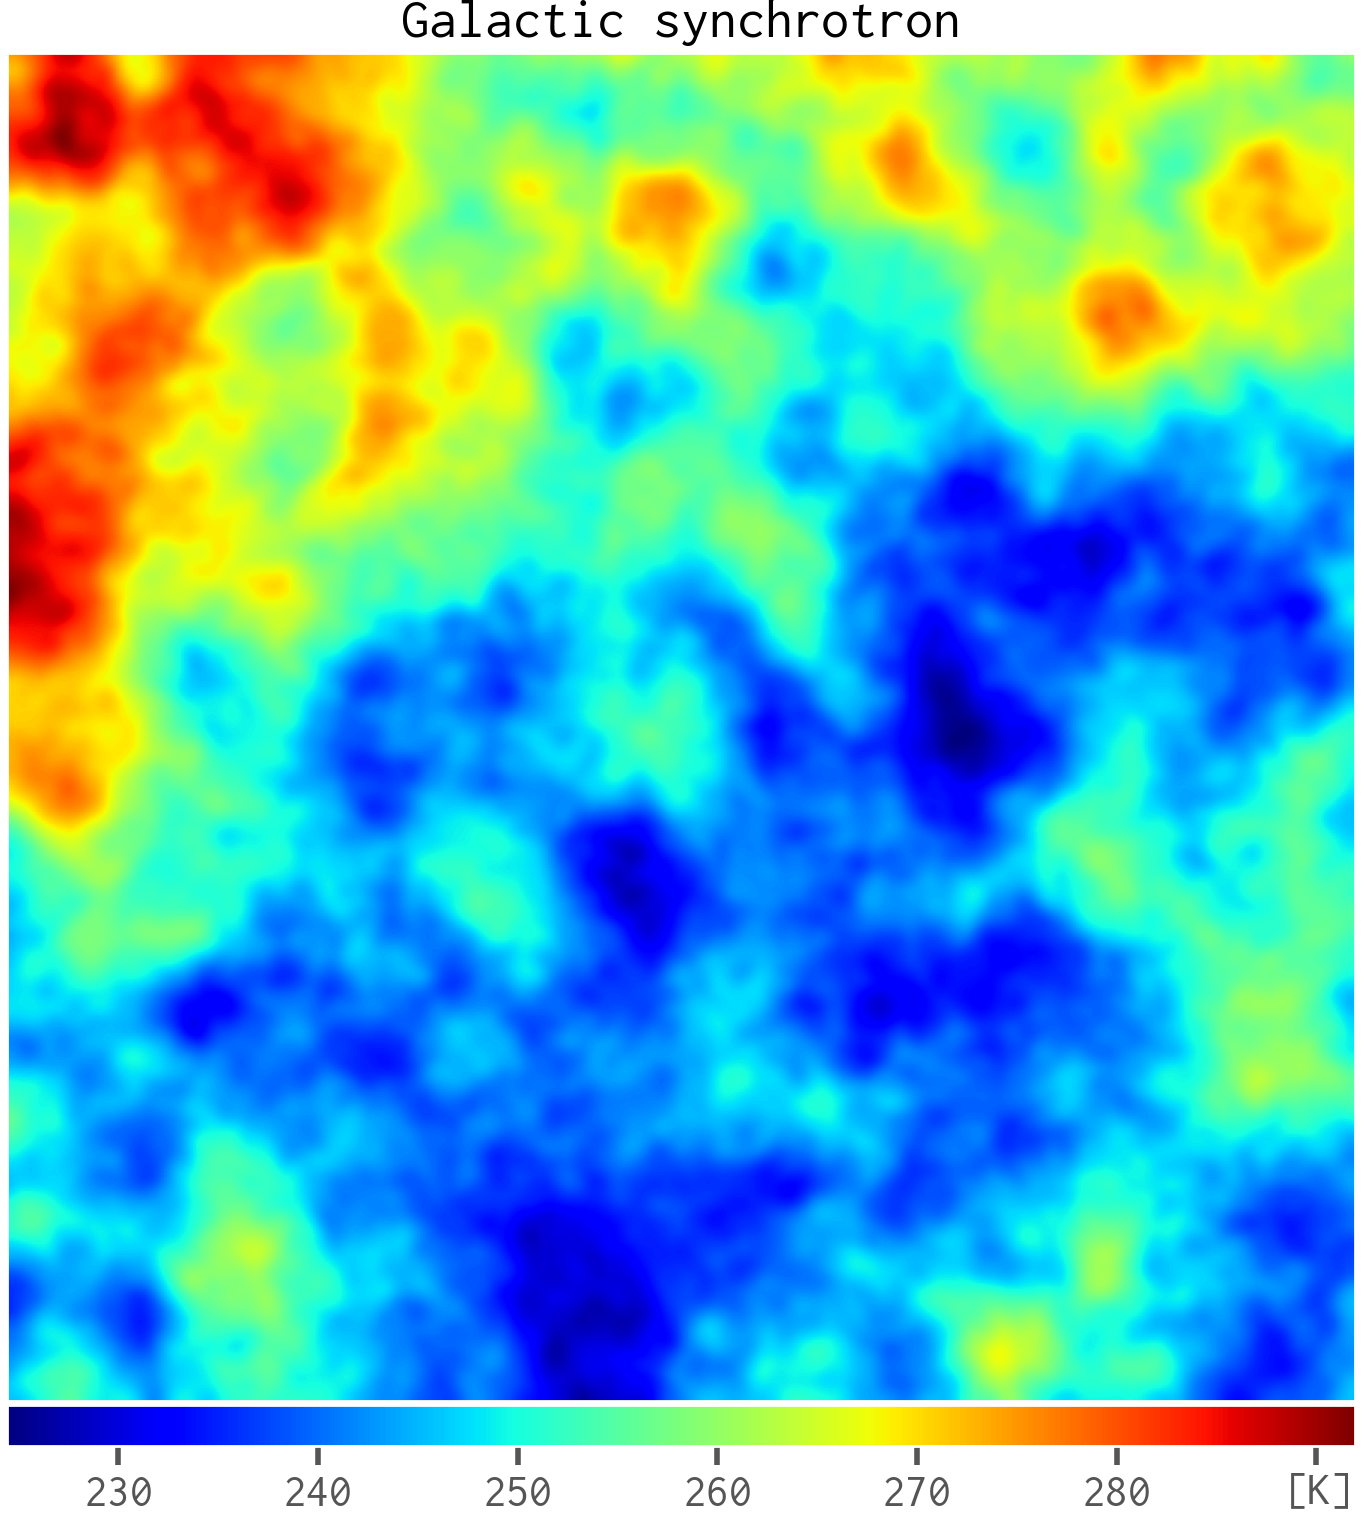
\includegraphics[width=0.498\textwidth]{skymap-gsyn-f158}%
  \hfill
  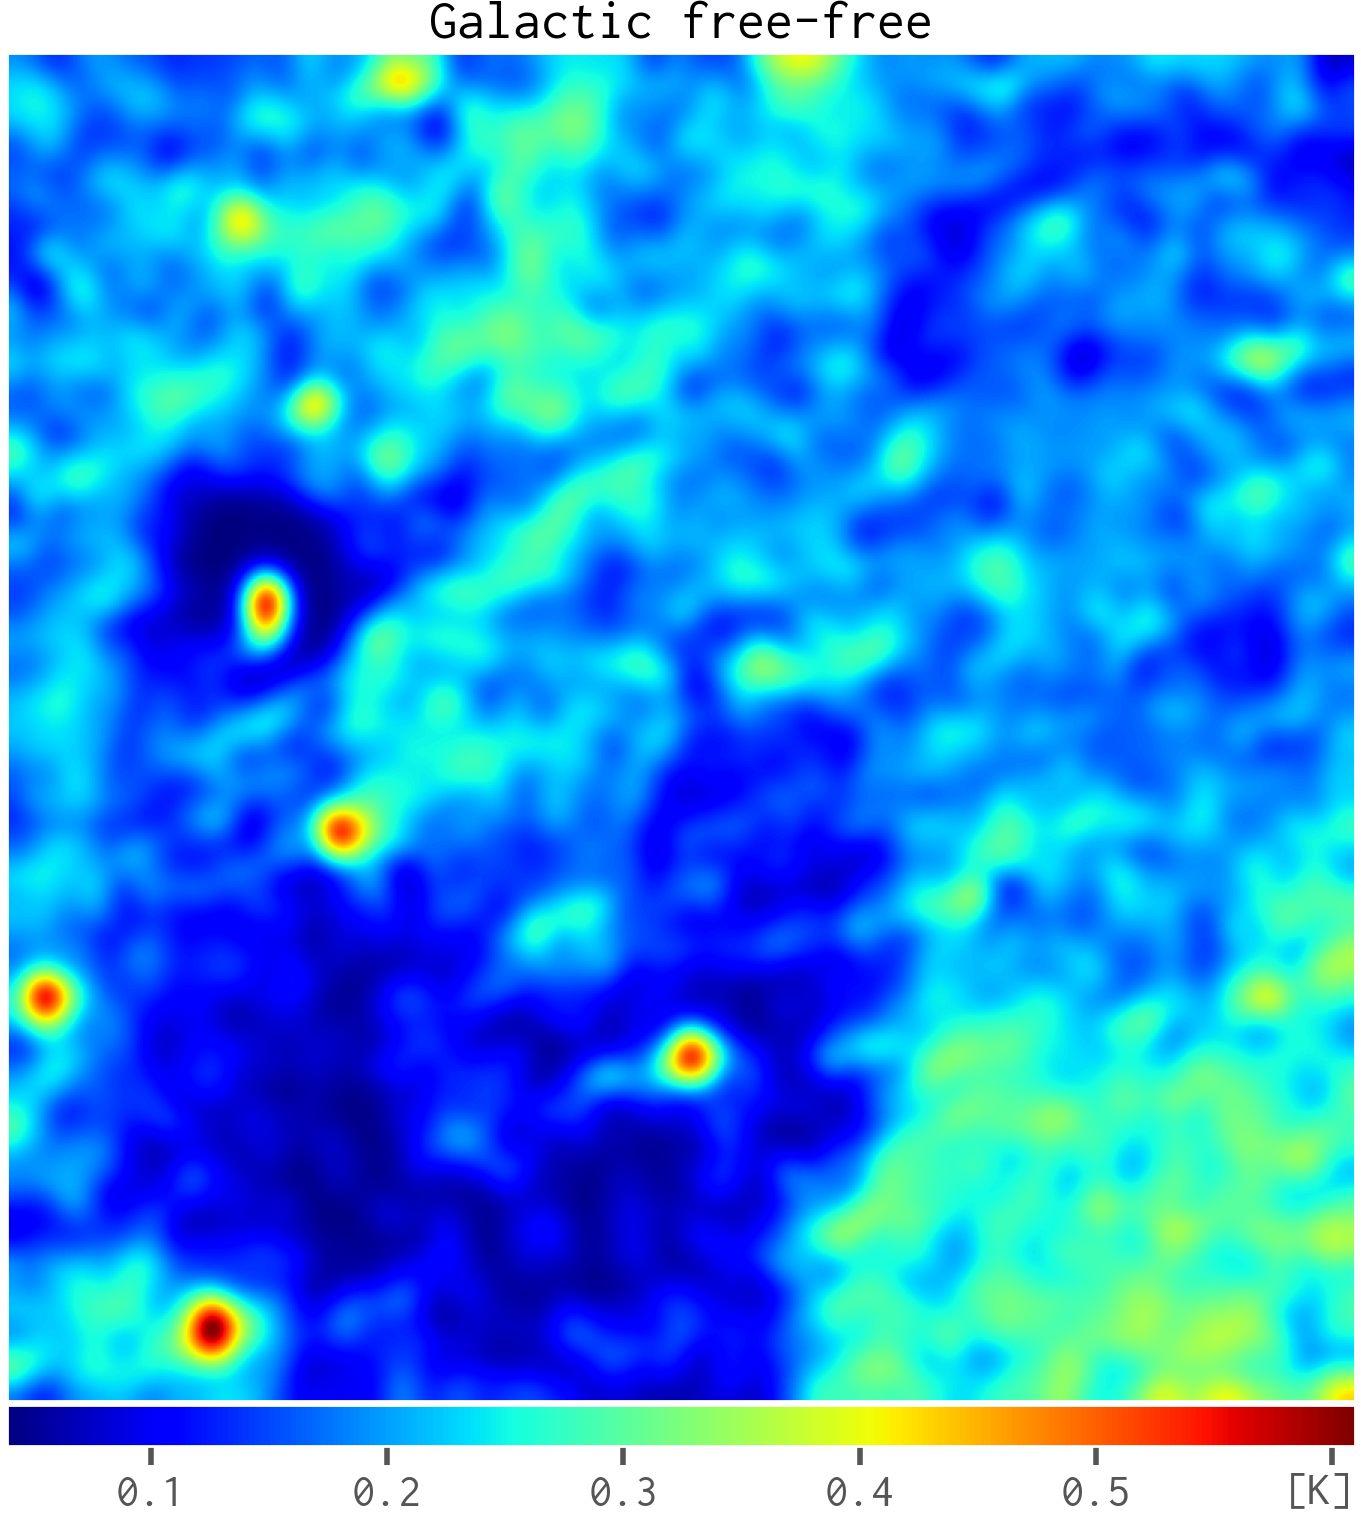
\includegraphics[width=0.498\textwidth]{skymap-gff-f158}
  \bicaption[银河系同步辐射和自由--自由辐射在 \SI{158}{\MHz} 的天图]{%
    TODO...
  }{%
    The sky maps of the Galactic synchrotron (left panel)
    and free-free (right panel) radiations at \SI{158}{\MHz}.
    Both maps have a sky region size of \SI{10 x 10}{\degree}
    and the color bars are in units of \si{\K}.
  }
  \label{fig:galactic-skymaps}
\end{figure}

%---------------------------------------------------------------------
\subsection{自由--自由辐射}
\label{sec:simu-gff}

TODO... simulation details...

The Galactic free-free emission is deduced from the Hα survey
data \cite{finkbeiner2003}, which is corrected for dust absorption,
by employing the tight relation between the Hα and free-free
emissions due to their common origins
(参考 \citeay{dickinson2003} 及其所引文献).
Since the Galactic diffuse emissions vary remarkably across the sky,
we simulate them at position of
(R.A., Dec.\@) = (\SI{0}{\degree}, \SI{-27}{\degree}), which locates at a
high galactic latitude ($b = \SI{-78.5}{\degree}$) and is expected to be
an appropriate choice for this study (see also \autoref{sec:obs-simu}).
\autoref{fig:galactic-skymaps} 右栏显示了银河系\ac{rad-ff}在 \SI{158}{\MHz} 的天图.


%=====================================================================
\section{河外点源}

TODO... simulation details

河外点源可大致分为以下几类 \cite{snellen2000,wilman2008,wang2010}:
(1) 恒星形成星系 (star-forming galaxy),
包括普通晚型星系 (normal late-type galaxy) 和星暴星系 (starburst galaxy);
(2) 射电宁静 (radio-quiet) \ac{agn};
(3) \ac{fr} I 型和 II 型 \ac{agn};
(4) GHz 倒转谱 (GHz-peaked-spectrum) \ac{agn};
(5) 致密陡谱 (compact steep-spectrum) \ac{agn}.

We simulate the former three types of sources by leveraging the simulation
results made by \citeay{wilman2008}, and simulate the latter two types
by employing their corresponding luminosity functions and spectral models.
More details can be found in \citeay{wang2010} and references therein.
\autoref{fig:ptrsrc-skymap} 显示了模拟的河外点源在 \SI{158}{\MHz} 的天图.

\begin{figure}[htp]
  \centering
  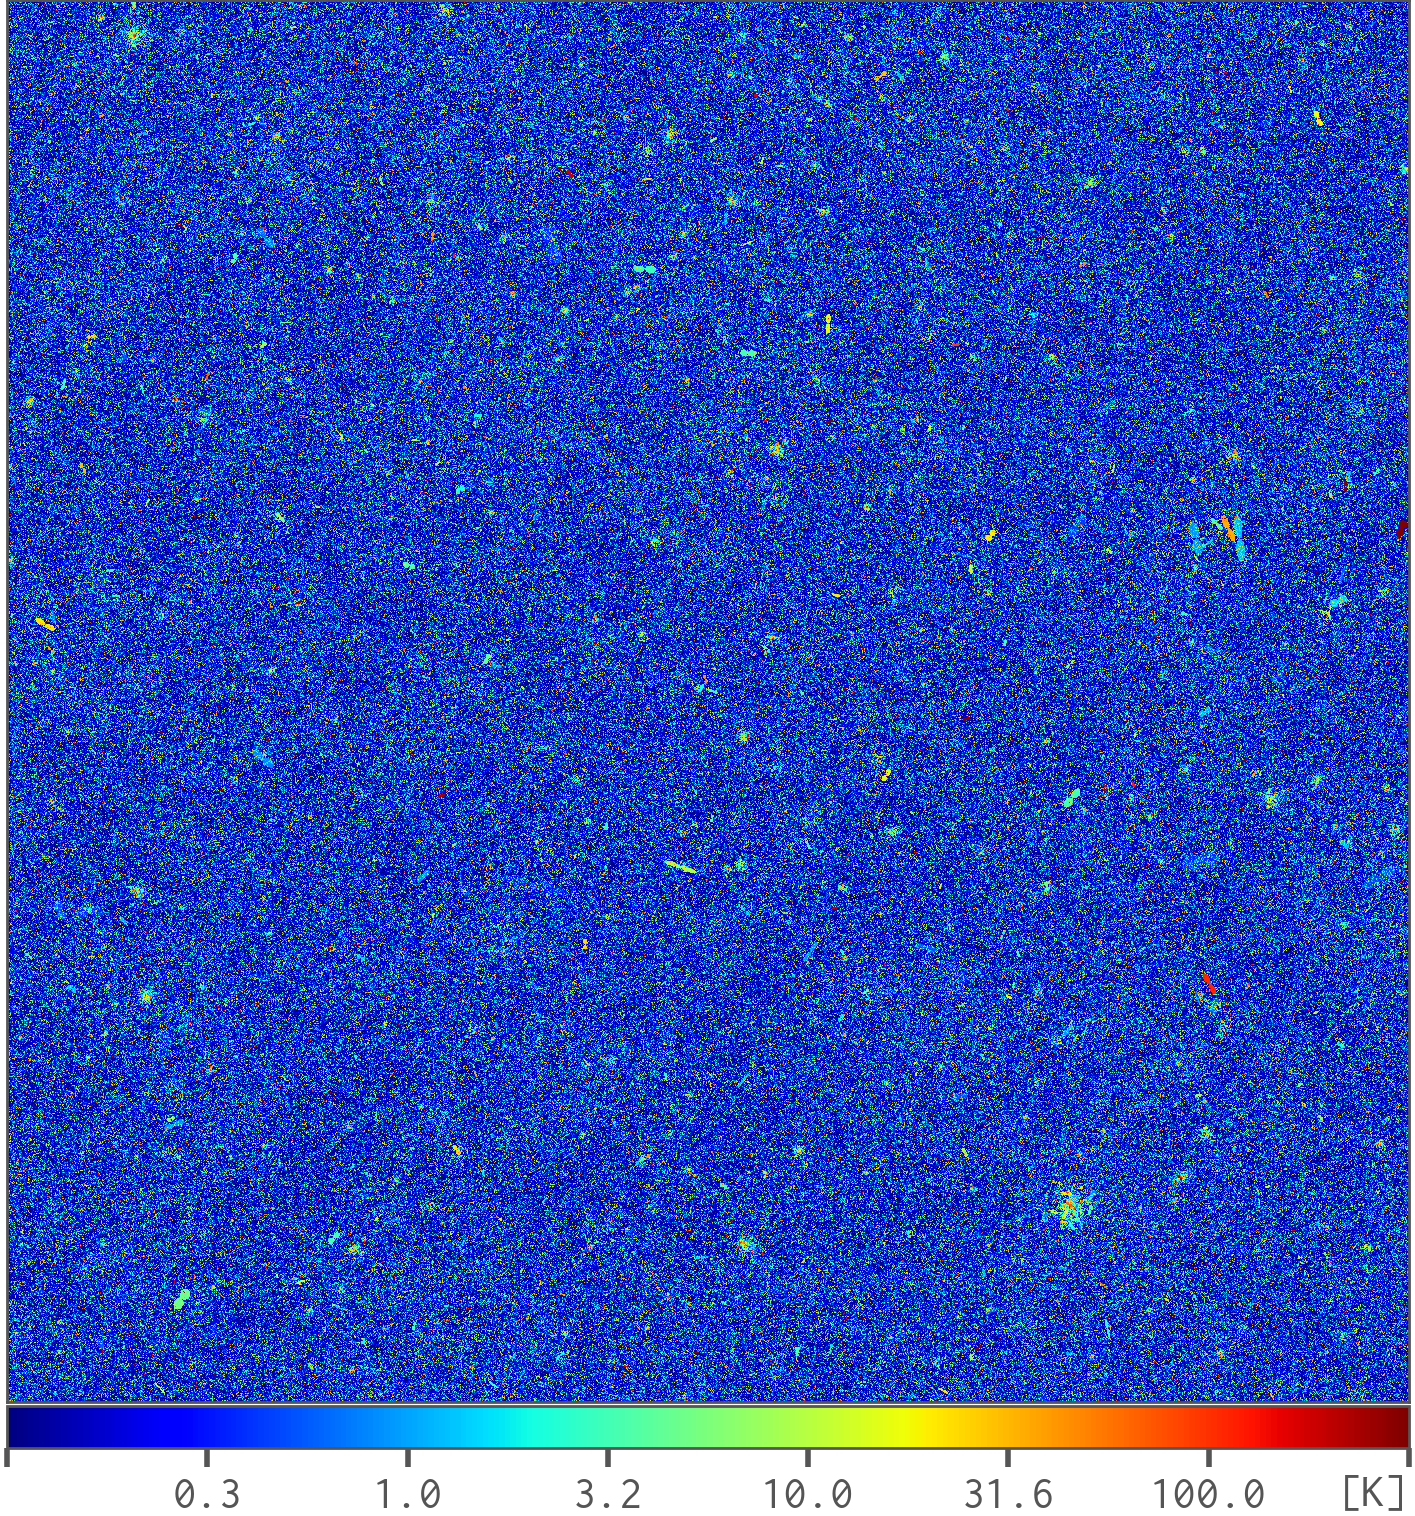
\includegraphics[width=0.7\textwidth]{skymap-ptrsrc-f158}
  \bicaption[河外点源在 \SI{158}{\MHz} 的模拟天图]{%
    TODO...
  }{%
    The simulated sky map of the extragalactic point sources at \SI{158}{\MHz}.
    The sky region size is \SI{10 x 10}{\degree}
    and the color bar is in units of \si{\K}.
  }
  \label{fig:ptrsrc-skymap}
\end{figure}


%=====================================================================
\section{EoR 信号}

The sky maps of the EoR signal are created using the 2016 data release
from the
\href{http://homepage.sns.it/mesinger/EOS.html}{Evolution Of 21\,cm Structure}
project\footnote{%
  Evolution Of 21\,cm Structure:
  \url{http://homepage.sns.it/mesinger/EOS.html}},
which has made use of the
\href{http://homepage.sns.it/mesinger/DexM___21cmFAST.html}{\texttt{21cmFAST}}%
\footnote{%
  21cmFAST: \url{http://homepage.sns.it/mesinger/DexM___21cmFAST.html}
} to simulate the cosmic
reionization process from redshift 86.5 to 5.0 inside a large cube that is
1.6 comoving \si{\Gpc} (1024 cells) along each side \cite{mesinger2016}.
We extract the image slices at needed frequencies (i.e., redshifts) from
the light-cone cubes of the recommended \enquote{faint galaxies} case,
and then tile and re-scale them to have the same sky coverage and
pixel size as our foreground maps.
\autoref{fig:eor-tbrms} shows the root-mean-square brightness temperatures of the
EoR signal among \SIrange{120}{200}{\MHz} ($z = \numrange{6.1}{10.8}$).
The corresponding root-mean-square brightness temperatures at the central
frequencies of the three adopted bands are given in \autoref{tab:tb-rms}
and the sky map of the EoR signal at \SI{158}{\MHz} is shown in
\autoref{fig:eor-skymap}.

\begin{figure}[htp]
  \centering
  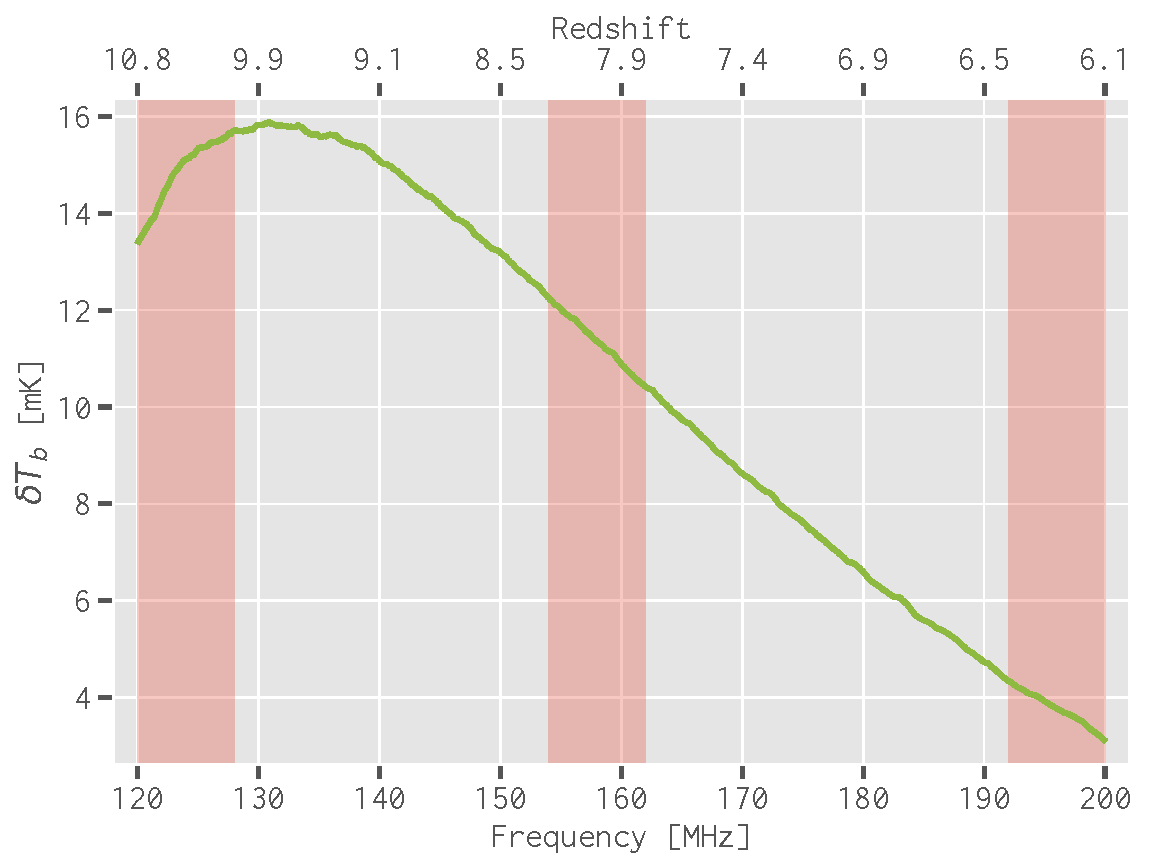
\includegraphics[width=0.8\textwidth]{eos2016-tbrms}
  \bicaption[EoR 信号在 \SIrange{120}{200}{\MHz} 的亮温度的\acs*{rms}值]{%
    TODO...
  }{%
    The root-mean-square brightness temperatures of the EoR signal
    (solid green line) within \SIrange{120}{200}{\MHz}
    ($z = \numrange{6.1}{10.8}$).
    The red shaded regions mark the three adopted frequency bands
    (\numrange{120}{128}, \numrange{154}{162}, and \numrange{192}{200}
    \si{\MHz}).
  }
  \label{fig:eor-tbrms}
\end{figure}

\begin{figure}[htp]
  \centering
  \includegraphics[width=0.7\textwidth]{skymap-eor-f158}
  \bicaption[EoR 信号在 \SI{158}{\MHz} 的天图]{%
    TODO...
  }{%
    The sky map of the EoR signal at \SI{158}{\MHz}.
    The sky region size is \SI{10 x 10}{\degree}
    and the color bar is in units of \si{\mK}.
  }
  \label{fig:eor-skymap}
\end{figure}


%=====================================================================
\section{干涉阵列的模拟观测}
\label{sec:obs-simu}

In order to properly evaluate the contamination of radio halos
on the EoR observations, it is essential to take account of the
practical instrumental effects of radio interferometers.

%---------------------------------------------------------------------
\subsection{SKA1-Low~阵列布局}

TODO: layout configuration, design goals, descriptions, figures...

Therefore, we employ the latest SKA1-Low layout configuration%
\footnote{\raggedright%
  SKA1-Low Configuration Coordinates:
  \url{https://astronomers.skatelescope.org/wp-content/uploads/2016/09/SKA-TEL-SKO-0000422_02_SKA1_LowConfigurationCoordinates-1.pdf}
  (released on 2016 May 21)
}
to simulate the SKA observations of the above simulated sky maps.
According to this layout configuration,
the SKA1-Low interferometer consists of 512 stations, with 224 of them
randomly distributed within the \enquote{core} of \SI{1000}{\meter} in
diameter, while the remaining stations are grouped into \enquote{clusters}
and placed on 3 spiral arms extending up to a radius of
\SI{\sim 35}{\kilo\meter}.
Each station has 256 antennas randomly distributed with a minimum separation
of $d_{\R{min}} = \SI{1.5}{\meter}$ inside a circular region of
\SI{35}{\meter} in diameter \cite{mort2017}.

%---------------------------------------------------------------------
\subsection{模拟观测和成像}

The \SI{8}{\MHz} bandwidth of each frequency band is divided into 51
channels for a frequency resolution of \SI{160}{\kilo\hertz}.
For each component, we simulate the input sky maps at every frequency
channel, and then use the
\href{https://github.com/OxfordSKA/OSKAR}{\texttt{OSKAR}}\footnote{%
  OSKAR: \url{https://github.com/OxfordSKA/OSKAR} (version 2.7.0)}
simulator \cite{mort2010} to perform observations for \SI{6}{\hour}.
The input sky maps are centered at sky position of
(R.A., Dec.\@) = (\SI{0}{\degree}, \SI{-27}{\degree}),
which passes through the zenith of the SKA1-Low telescope and
is an ideal choice for the simulation of SKA observations.
The simulated visibility data are imaged through the
\href{https://sourceforge.net/p/wsclean}{\texttt{WSClean}}\footnote{%
  WSClean: \url{https://sourceforge.net/p/wsclean} (version 2.6)}
imager \cite{offringa2014} using Briggs' weighting with a
robustness of zero \cite{briggs1995},
and the created images are cropped to keep only the central regions
because the marginal regions suffer from the problem of insufficient
CLEAN.
As the telescope's field of view (FoV) is inversely proportional to
the observing frequency, we choose to keep the central
\SI{6 x 6}{\degree}, \SI{5 x 5}{\degree}, and \SI{4 x 4}{\degree}
regions in the \numrange{120}{128}, \numrange{154}{162}, and
\numrange{192}{200} \si{\MHz} frequency bands, respectively.

The Galactic synchrotron and free-free emissions are combined for the
simulated observations because they have similar diffuse features.
Similar to the real-time peeling of the brightest point sources in
practical data analysis pipelines
\cite{mitchell2008,intema2009,mort2017},
we assume that extragalactic point sources with a \SI{158}{\MHz} flux
density $S_{158} > \SI{50}{\mJy}$ are removed
\cite{liu2009ps,pindor2011}.
Thus, the root-mean-square brightness temperatures of point sources
are significantly reduced to be about
\num{22.5e4}, \num{9.81e4}, and \num{4.75e4} \si{\mK}
at 124, 158, and 196 \si{\MHz}, respectively.
In addition, we create the foreground image cubes in each frequency band
using the CLEAN algorithm with joined-channel deconvolution in order
to ensure the spectral smoothness \cite{offringa2017}, which is crucial
to extract the faint EoR signal in the presence of overwhelming
foreground contamination.
For the EoR signal, we directly use the dirty images because the CLEAN
algorithm is not well applicable to such faint and diffuse emissions.
Hence we obtain the SKA \enquote{observed} image cubes of the EoR signal,
radio halos, the Galactic diffuse emission (with synchrotron and
free-free emissions combined), and the extragalactic point sources
(with the brightest ones removed) in the \numrange{120}{128},
\numrange{154}{162}, and \numrange{192}{200} \si{\MHz} frequency bands.


%=====================================================================
\section{小结}

TODO


%% EOF
